\documentclass[journal,11pt,draftcls,onecolumn]{IEEEtran}
%\documentclass[journal,10pt,twocolumn,twoside]{IEEEtran}

\usepackage{graphicx}
\usepackage{amsmath, amsthm, amssymb, amsfonts, cancel}
\usepackage{algorithm, algorithmic, ifsym, subfigure}


% Alter some LaTeX defaults for better treatment of figures:
    % See p.105 of "TeX Unbound" for suggested values.
    % See pp. 199-200 of Lamport's "LaTeX" book for details.
    %   General parameters, for ALL pages:
    \renewcommand{\topfraction}{0.9}	% max fraction of floats at top
    \renewcommand{\bottomfraction}{0.8}	% max fraction of floats at bottom
    %   Parameters for TEXT pages (not float pages):
    \setcounter{topnumber}{2}
    \setcounter{bottomnumber}{2}
    \setcounter{totalnumber}{4}     % 2 may work better
    \setcounter{dbltopnumber}{2}    % for 2-column pages
    \renewcommand{\dbltopfraction}{0.9}	% fit big float above 2-col. text
    \renewcommand{\textfraction}{0.07}	% allow minimal text w. figs
    %   Parameters for FLOAT pages (not text pages):
    \renewcommand{\floatpagefraction}{0.7}	% require fuller float pages
	% N.B.: floatpagefraction MUST be less than topfraction !!
    \renewcommand{\dblfloatpagefraction}{0.7}	% require fuller float pages

	% remember to use [htp] or [htpb] for placement

%\def\BibTeX{{\rm B\kern-.05em{\sc i\kern-.025em b}\kern-.08em
%    T\kern-.1667em\lower.7ex\hbox{E}\kern-.125emX}}
\def\Var{{\rm Var}}
\def\Cov{{\rm Cov}}
\def\tr{{\rm tr}}
\def\E{{\rm E}}
\def\P{{\rm P}}
\def\bA{ {\mathbf{A}} }
\def\bB{ {\mathbf{B}} }
\def\bC{ {\mathbf{C}} }
\def\bD{ {\mathbf{D}} }
\def\bE{ {\mathbf{E}} }
\def\bF{ {\mathbf{F}} }
\def\bG{ {\mathbf{G}} }
\def\bH{ {\mathbf{H}} }
\def\bI{ {\mathbf{I}} }
\def\bJ{ {\mathbf{J}} }
\def\bK{ {\mathbf{K}} }
\def\bL{ {\mathbf{L}} }
\def\bM{ {\mathbf{M}} }
\def\bN{ {\mathbf{N}} }
\def\bO{ {\mathbf{O}} }
\def\bP{ {\mathbf{P}} }
\def\bQ{ {\mathbf{Q}} }
\def\bR{ {\mathbf{R}} }
\def\bS{ {\mathbf{S}} }
\def\bT{ {\mathbf{T}} }
\def\bU{ {\mathbf{U}} }
\def\bV{ {\mathbf{V}} }
\def\bW{ {\mathbf{W}} }
\def\bX{ {\mathbf{X}} }
\def\bY{ {\mathbf{Y}} }
\def\bZ{ {\mathbf{Z}} }

\def\bTheta{ {\mathbf{\Theta}} }
\def\bSigma{ {\mathbf{\Sigma}} }
\def\bDelta{ {\mathbf{\Delta}} }
\def\bXi{ {\mathbf{\Xi}} }

\def\nn{{ \parallel   }}
\def\RR{{ \mathbb{R}  }}
\def\PP{{ \mathbb{P}  }}
\def\NN{{ \mathbb{N}  }}
\def\vec{{ \text{vec} }}
\def\tr{{ \text{tr}   }}
\def\bdiag{{ \text{bdiag}   }}
\def\diag{{ \text{diag}   }}
\def\corr{{ \text{corr}   }}
\def\bx{{ \mathbf{x}  }}
\def\by{{ \mathbf{y}  }}
\def\bz{{ \mathbf{z}  }}
\def\bv{{ \mathbf{v}  }}
\def\card{{ \text{card} }}
\def\erf{{ \text{erf} }}
\def\sgn{{ \text{sgn} }}

\newtheorem{example}{Example}
\newtheorem{theorem}{Theorem}
\newtheorem{lemma}{Lemma}
\newtheorem{remark}{Remark}
\newtheorem{corollary}{Corollary}
\newtheorem{proposition}{Proposition}
\newtheorem{assumption}{Assumption}
\newtheorem{definition}{Definition}
\newtheorem{conjecture}{Conjecture}
\newtheorem{property}{Property}

\setcounter{page}{1}

\begin{document}
\title{On Convergence of Kronecker Graphical Lasso Algorithms}
\author{Theodoros Tsiligkaridis *, \textit{Student Member, IEEE}, Alfred O. Hero III, \textit{Fellow, IEEE}, Shuheng Zhou, \textit{Member, IEEE}}

\maketitle

\begin{abstract}
This paper presents a thorough convergence analysis of 
Kronecker graphical lasso (KGLasso) algorithms for estimating the covariance of an i.i.d. Gaussian random sample under a sparse Kronecker-product covariance model. The KGlasso model, originally called the transposable regularized covariance model by Allen {\it et al}  \cite{AllenTib10}, implements a pair of $\ell_1$ penalties on each Kronecker factor to enforce sparsity in the covariance estimator.   The KGlasso algorithm generalizes Glasso, introduced by Yuan and Lin \cite{YL07} and Banerjee {\it et al} \cite{ModelSel}, to estimate covariances having Kronecker product form.   It  also generalizes  the unpenalized ML flip-flop (FF) algorithm of Werner {\it et al} \cite{EstCovMatKron} to estimation of sparse Kronecker factors. %We establish that the KGlasso iterates converge pointwise to a local maximum of the penalized likelihood function.
We establish high dimensional rates of convergence to the true covariance as both the number of samples and the number of variables go to infinity. Our results establish that KGlasso has significantly faster asymptotic convergence than Glasso and FF. Simulations are presented that validate the results of our analysis.  For example, for a sparse $10,000 \times 10,000$ covariance matrix equal to the Kronecker product of two $100 \times 100$ matrices, the root mean squared error of the inverse covariance estimate using FF is 3.5 times larger than that obtainable using KGlasso.
\end{abstract} 

\begin{keywords}
	Sparsity, structured covariance estimation, penalized maximum likelihood, graphical lasso, direct product representation.
\end{keywords}


\section{Introduction}
Covariance estimation is a problem of great interest in many different disciplines, including machine learning, signal processing, economics and bioinformatics. In many applications the number of variables is very large, e.g., in the tens or hundreds of thousands, leading to a number of covariance parameters that greatly exceeds the number of observations.  To address this problem constraints are frequently imposed on the covariance to reduce the number of parameters in the model. For example, the Glasso model of  Yuan and Lin \cite{YL07} and Banerjee {\it et al} \cite{ModelSel}  imposes sparsity constraints on the covariance. The Kronecker product  model of Werner {\it et al} \cite{EstCovMatKron} assumes that the covariance can be represented as the Kronecker product  of two lower dimensional covariance matrices. The 
transposable regularized covariance model of Allen {\it et al}  \cite{AllenTib10} imposes a combination of sparsity and Kronecker product form on the covariance. When there is no missing data, an extension of the alternating optimization algorithm of  \cite{EstCovMatKron}, called the flip flop (FF) algorithm, can be applied to estimate the parameters of this combined sparse and Kronecker product model.  In this paper we call this algorithm the Kronecker Glasso (KGlasso) and  we thoroughly analyze convergence of the algorithm in the high dimensional setting.  


As in \cite{EstCovMatKron} we assume that there are $pf$ variables whose covariance $\mathbf{\Sigma}_0$ has the separable positive definite Kronecker product representation:
\begin{equation} \label{factorize}
	\mathbf{\Sigma}_{0} = \mathbf{A}_0 \otimes \mathbf{B}_0
\end{equation}
where $\bA_0$ is a $p\times p$ positive definite matrix and $\bB_0$ is an $f \times f$ positive definite matrix.  This model (\ref{factorize}) is relevant to channel modeling for MIMO wireless communications, where $\bA_0$ is a transmit covariance matrix and $\bB_0$ is a receive covariance matrix \cite{MIMOWerner}. The model is also relevant to other transposable models arising in recommendation systems like NetFlix and in gene expression analysis \cite{AllenTib10}. 
The Kronecker factorization (\ref{factorize}) can easily be generalized to the $k$-fold case, where $\mathbf{\Sigma}_0=\mathbf{A}_1\otimes \mathbf{A}_2 \otimes \dots \otimes \mathbf{A}_k$. 

Under the assumption that the measurements are multivariate Gaussian with covariance having the Kronecker product form (\ref{factorize}), the maximum likelihood (ML) estimator can be formulated \cite{LuZimmerman2}. While the ML estimator has no known closed-form solution, an approximation to the solution can be iteratively computed via an alternating algorithm: the flip-flop (FF) algorithm \cite{LuZimmerman2, EstCovMatKron}.  As compared to the standard saturated (unstructured) covariance model, the number of unknown parameters in (\ref{factorize}) is reduced from order $\Theta(p^2 f^2)$ to order $\Theta(p^2)+\Theta(f^2)$.
This results in a significant reduction in the mean squared error (MSE) and the computational complexity of the maximum likelihood (ML) covariance estimator. This paper establishes that further reductions MSE are achievable when the Kronecker matrix factors are known to have sparse inverses, i.e., the measurements obey a sparse Kronecker structured Gaussian graphical model.

The graphical lasso (Glasso) estimator was originally proposed in \cite{YL07, ModelSel} for estimating a sparse inverse covariance, also called the precision matrix, under an i.i.d. Gaussian observation model. An algorithm for efficiently solving the nonsmooth optimization problem that arises in the Glasso estimator, based on ideas from \cite{ModelSel}, was proposed in \cite{Glasso}. Glasso has been applied to the time-varying coefficients setting in Zhou {\it et al} \cite{TimeVaryingGraphs} using the kernel estimator for covariances at a target time. Rothman {\it et al} \cite{Rothman} derived high dimensional convergence rates for a slight variant of Glasso, i.e., only the off-diagonal entries of the estimated precision matrix were penalized using an $\ell_1$-penalty. The high dimensional convergence rate of Glasso was established by Ravikumar {\it et al}  \cite{RWRY08}. This paper extends their analysis to the case that the covariance has Kronecker structure (\ref{factorize}), showing that significantly higher rates of convergence are achievable.


%The first contribution of this paper is proof that the KGlasso iterations converge to a local maximum of the KGlasso objective function for fixed number of samples $n$ and fixed matrix dimensions $p$ and $f$.
%
The main contribution is the derivation of the high-dimensional MSE convergence rates for KGlasso as $n$, $p$ and $f$ go to infinity.
 When both Kronecker factors are sparse, it is shown that KGlasso \textit{strictly} outperforms FF and Glasso in terms of MSE convergence rate. More specifically, we show KGlasso achieves a convergence rate of $O_P\left(\frac{(p+f)\log \max(p,f,n)}{n}\right)$ and FF achieves a rate of $O_P\left(\frac{(p^2+f^2)\log \max(p,f,n)}{n}\right)$ as $n\to\infty$, while it is known \cite{Rothman, TimeVaryingGraphs} that Glasso achieves a rate of $O_P\left(\frac{(pf+s)\log \max(p,f,n)}{n}\right)$, where $s$ denotes the number of off-diagonal nonzero elements in the true precision matrix $\bTheta_0$. Simulations show that the performance improvements predicted by the high-dimensional analysis continue to hold for small sample size and moderate matrix dimension. For the example studied in Sec. \ref{sec: simulations} the empirical MSE of KGlasso is significantly lower than that of Glasso and FF for $p=f=100$ over the range of $n$  from $10$ to $100$.


The starting point for the MSE convergence analysis is the large-sample analysis of the FF algorithm (Thm. 1 in \cite{EstCovMatKron}). The KGlasso convergence proof uses a large deviation inequality  that shows that the dimension of one estimated Kronecker factor, say $\bA$, acts as a multiplier on the number of independent samples when performing inference on the other factor $\bB$. This result is then used to obtain optimal MSE rates in terms of Frobenius norm error between the KGlasso estimated matrix and the ground truth. The asymptotic MSE convergence analysis is useful since it can be used to guide the selection of sparsity regularization parameters and to determine minimum sample size requirements.

The outline of the paper is as follows. Section \ref{sec: notation} introduces the notation that will be used throughout the paper. In Section \ref{sec: glasso}, the graphical lasso framework is introduced. Section \ref{sec: algorithm} uses this framework to introduce the KGlasso algorithm. Section \ref{sec: convergence_analysis_KGL} shows convergence of KGlasso and characterizes its limit points. The high dimensional MSE convergence rate derivation for the FF algorithm is included in Section \ref{sec: FF_rate}. Section \ref{sec: consistency} presents a high-dimensional MSE rate result that is used to establish the superiority of KGlasso as compared to FF and standard Glasso, under the sparse Kronecker product representation (\ref{factorize}). Section \ref{sec: simulations} presents simulations that empirically validate the theoretical convergence rates obtained in Section \ref{sec: consistency}.


\section{Notation} \label{sec: notation}
For a square matrix $\mathbf{M}$, define $|\mathbf{M}|_1=\nn \vec(\mathbf{M}) \nn_1$ and $|\mathbf{M}|_\infty=\nn \vec(\mathbf{M}) \nn_\infty$, where $\vec(\mathbf{M})$ denotes the vectorized form of $\mathbf{M}$ (concatenation of columns into a vector). $\nn \mathbf{M} \nn_2$ is the spectral norm of $\bM$. $\mathbf{M}_{i,j}$ and $[\mathbf{M}]_{i,j}$ are the $(i,j)$th element of $\mathbf{M}$. Let the inverse transformation (from a vector to a matrix) be defined as: $\vec^{-1}(\mathbf{x})=\mathbf{X}$, where $\mathbf{x}=\vec(\mathbf{X})$. Define the $pf\times pf$ permutation operator $\bK_{p,f}$ such that $\bK_{p,f} \vec(\bN) = \vec(\bN^T)$ for any $p\times f$ matrix $\bN$. For a symmetric matrix $\mathbf{M}$, $\lambda(\mathbf{M})$ will denote the vector of real eigenvalues of $\mathbf{M}$ and define $\lambda_{max}(\mathbf{M})=\nn\bM \nn_2=\max{\lambda_i(\mathbf{M})}$ for p.d. symmetric matrix, and $\lambda_{min}(\mathbf{M}) = \min{\lambda_i(\mathbf{M})}$. Define the sparsity parameter associated with $\bM$ as $s_{M}=\card(\{(i_1,i_2): [\bM]_{i_1,i_2}\neq 0, i_1\neq i_2 \})$. Let $\kappa(\bM):=\frac{\lambda_{max}(\bM)}{\lambda_{min}(\bM)}$ denote the condition number of a symmetric matrix $\bM$.

For a matrix $\bM$ of size $pf\times pf$, let $\{\bM(i,j)\}_{i,j=1}^p$ denote its $f\times f$ block submatrices, where each block submatrix is $\bM(i,j)=[\bM]_{(i-1)f+1:if,(j-1)f+1:jf}$. Also let $\{\overline{\bM}(k,l)\}_{k,l=1}^f$ denote the $p\times p$ block submatrices of the permuted matrix $\overline{\bM}=\bK_{p,f}^T \bM \bK_{p,f}$.

Define the set of symmetric matrices $S^p = \{\mathbf{A}\in \RR^{p\times p}: \mathbf{A}=\mathbf{A}^T\}$, the set of symmetric positive semidefinite (psd) matrices $S_{+}^p$, and the set of symmetric positive definite (pd) matrices $S_{++}^p$. $\bI_d$ is a $d\times d$ identity matrix. It can be shown that $S_{++}^p$ is a convex set, but is not closed \cite{ConvexOpt}. Note that $S_{++}^p$ is simply the interior of the closed convex cone $S_{+}^p$.

Statistical convergence rates will be denoted by the $O_P(\cdot)$ notation, which is defined as follows. Consider a sequence of real random variables $\{X_n\}_{n \in \NN}$ defined on a probability space $(\Omega,\mathcal{F},P)$ and a deterministic (positive) sequence of reals $\{b_n\}_{n\in \NN}$. By $X_n=O_P(1)$ is meant: $\sup_{n\in \NN}{\Pr(|X_n|>K)} \to 0$ as $K\to\infty$, where $\bX_n$ is a sequence indexed by $n$, for fixed $p,f$. %for all $\epsilon>0$, $\exists M=M(\epsilon)<\infty$ such that $\sup_{n\in \NN}{P(|X_n|>M)} < \epsilon$.
The notation $X_n=O_P(b_n)$ is equivalent to $\frac{X_n}{b_n}=O_P(1)$. By $X_n=o_p(1)$ is meant $\Pr(|X_n|>\epsilon) \to 0$ as $n\to\infty$ for any $\epsilon>0$. By $\lambda_n \asymp b_n$ is meant $c_1 \leq \frac{\lambda_n}{b_n} \leq c_2$ for all $n$, where $c_1,c_2>0$ are absolute constants.



\section{Graphical Lasso Framework} \label{sec: glasso}
For simplicity, we assume the number of Kronecker components is $k=2$. Available are $n$ i.i.d. multivariate Gaussian observations $\{\bz_t\}_{t=1}^{n}$, where $\bz_t\in \RR^{pf}$, having zero-mean and covariance equal to $\mathbf{\Sigma} = \mathbf{A}_0 \otimes \mathbf{B}_0$. Then, ignoring irrelevant constants,  the log-likelihood  $l(\mathbf{\Sigma})$ is:
\begin{equation} \label{log_likelihood}
	l(\mathbf{\Sigma}) = \log\det(\mathbf{\Sigma}^{-1}) - \tr(\mathbf{\Sigma}^{-1}\hat{\mathbf{S}}_n),
\end{equation}
where $\mathbf{\Sigma}$ is the positive definite covariance matrix and $\hat{\mathbf{S}}_n=\frac{1}{n}\sum_{t=1}^{n}{\bz_t \bz_t^T}$ is the sample covariance matrix. Recent work \cite{ModelSel, Glasso, RWRY08} has considered $\ell_1$-penalized maximum likelihood estimators for the saturated model where $\bSigma$ belongs to the unrestricted cone of positive definite matrices. These estimators are known as graphical lasso (Glasso) estimators and are obtained as the solution to the $\ell_1$-penalized minimization problem:
\begin{equation} \label{opt_prob}
	\hat{\mathbf{\Sigma}}_n \in \arg \min_{\mathbf{\Sigma} \in S_{++}^p} { \{ -l(\mathbf{\Sigma}) + \lambda |\mathbf{\Sigma}^{-1}|_1 \} },
\end{equation}
where $\lambda \geq 0$ is a regularization parameter. If $\lambda>0$ and $\hat{\mathbf{S}}_n$ is positive definite, then $\hat{\mathbf{\Sigma}}_n$ in (\ref{opt_prob}) is the unique minimizer.

A fast iterative algorithm, based on a block coordinate descent approach, exhibiting a computational complexity $\mathcal{O}((pf)^3)$, was developed in \cite{Glasso} to solve the convex program (\ref{opt_prob}). Under the assumption $\lambda \asymp \sqrt{\frac{\log(pf)}{n}}$ solution of (\ref{opt_prob}) was shown to have high dimensional convergence rate \cite{Rothman, TimeVaryingGraphs}:
\begin{equation} \label{Glasso_rate}
 \nn \bG(\hat{\bS}_n, \lambda)-\bTheta_0 \nn_F = O_P\left( \sqrt{\frac{(pf+s) \log(pf)}{n}} \right)
\end{equation}
where $s$ is an upper bound on the number of non-zero off-diagonal elements of $\bTheta_0$. When $s=O(pf)$, this rate is better than that achieved in the case of the standard sample covariance estimator ($\lambda=0$):
\begin{equation} \label{naive_SCM_rate}
	\nn \hat{\bS}_n - \bSigma_0 \nn_F = O_P\left( \sqrt{\frac{p^2f^2}{n}} \right).
\end{equation}



\section{Kronecker Graphical Lasso} \label{sec: algorithm}
Let $\mathbf{\Sigma}_0=\mathbf{A}_0 \otimes \mathbf{B}_0$ denote the true covariance matrix, where $\mathbf{A}_0=\mathbf{X}_0^{-1}$ and $\mathbf{B}_0=\mathbf{Y}_0^{-1}$ are the true Kronecker factors. Let $\mathbf{A}_{init}$ denote an initial guess of $\mathbf{A}_0=\mathbf{X}_0^{-1}$.

Define $J(\bX,\bY)$ as the negative log-likelihood
\begin{align}
	J(\bX,\bY) &= \tr((\bX \otimes \bY)\hat{\bS}_n) - f \log\det(\bX) \nonumber \\
		& \quad -p \log\det(\bY) \label{J_func_2}
\end{align}
Although the objective function (\ref{J_func_2}) is not jointly convex in $(\bX, \bY)$, it is biconvex. This motivates the flip-flop algorithm \cite{EstCovMatKron}. 
%
Adapting the notation from \cite{EstCovMatKron}, define the mappings $\hat{\mathbf{A}}(\cdot), \hat{\mathbf{B}}(\cdot)$:
\begin{align}
	\underbrace{\hat{\mathbf{A}}(\mathbf{B})}_{p\times p} &= \frac{1}{f} \sum_{k,l=1}^f{[\mathbf{B}^{-1}]_{k,l}\overline{\hat{\mathbf{S}}_n}(l,k)}, \label{A_update} \\
	\underbrace{\hat{\mathbf{B}}(\mathbf{A})}_{f\times f} &= \frac{1}{p} \sum_{i,j=1}^p{[\mathbf{A}^{-1}]_{i,j} \hat{\mathbf{S}}_n(j,i)}, \label{B_update}
\end{align}
where $\overline{\hat{\bS}}_n=\bK_{p,f}^T \hat{\bS}_n \bK_{p,f}$ (see Sec. \ref{sec: notation} for definition of $K_{p,f}$). For fixed $\bB\in S_{++}^f$, $\hat{\bA}(\bB)$ in (\ref{A_update}) is the minimizer of $J(\bA^{-1},\bB^{-1})$ over $\bA\in S_{++}^p$. A similar interpretation holds for (\ref{B_update}). The flip-flop algorithm starts with some arbitrary p.d. matrix $\bA_{init}$ and computes $\bB$ using (\ref{B_update}), then $\bA$ using (\ref{A_update}), and repeats until convergence. This algorithm does not account for sparsity.

If $\bTheta_0=\bX_0\otimes \bY_0$ is a sparse matrix, which implies that at least one of $\bX_0$ or $\bY_0$ is sparse, one can penalize the outputs of the flip-flop algorithm and minimize
\begin{equation} \label{J_lambda_func}
	J_\lambda(\bX,\bY) = J(\bX,\bY) + \bar{\lambda}_X |\bX|_1 + \bar{\lambda}_Y |\bY|_1 .
\end{equation}
where $\bar{\lambda}_X=\lambda_X/f$ and $\bar{\lambda}_Y=\lambda_Y/p$. This leads to an algorithm that we call KGlasso (see Algorithm \ref{alg: algKGL}), which sparsifies the Kronecker factors in proportion to the parameters $\bar{\lambda}_X, \bar{\lambda}_Y >0$. This is the same objective function that was proposed in \cite{AllenTib10} when specialized to the case that there is no missing data.

\begin{algorithm}
\caption{Kronecker Graphical Lasso (KGlasso) }
\label{alg: algKGL}
\begin{algorithmic}[1]
\STATE \textbf{Input:}  {$\hat{\bS}_n$, $p$, $f$, $n$, $\bar{\lambda}_X >0$, $\bar{\lambda}_Y >0$}
\STATE \textbf{Output:} {$\hat{\bTheta}_{KGlasso}$}

	\STATE Initialize $\bA_{init}$ to be positive definite satisfying Assumption \ref{assumption_posdef_unif}.
	\STATE $\check{\bX} \leftarrow \bA_{init}^{-1}$
	
	\REPEAT
	  \STATE	$\hat{\bB} \leftarrow \frac{1}{p} \sum_{i,j=1}^p{[\check{\bX}]_{i,j} \hat{\bS}_n(j,i)}$ (see Eq. (\ref{A_update}))
  	\STATE  $\check{\bY} \leftarrow \bG(\hat{\bB}, \frac{\bar{\lambda}_Y}{p})$, where $\bG(\cdot,\cdot)$ is defined in (\ref{G_operator})
  	\STATE  $\hat{\bA} \leftarrow \frac{1}{f} \sum_{k,l=1}^f{[\check{\bY}]_{k,l} \overline{\hat{\bS}_n}(l,k)}$ (see Eq. (\ref{B_update}))
  	\STATE  $\check{\bX} \leftarrow \bG(\hat{\bA}, \frac{\bar{\lambda}_X}{f})$
	\UNTIL {convergence}
	
	\STATE $\hat{\bTheta}_{KGlasso} \leftarrow \check{\bX} \otimes \check{\bY}$
\end{algorithmic}
\end{algorithm}


The Glasso mapping (\ref{opt_prob}) is written as $\bG(\cdot,\lambda): S^d \to S^d$,
\begin{equation} \label{G_operator}
	\bG(\bT,\lambda) = \arg\min_{\bTheta \in S_{++}^d} \Big\{ \tr(\bTheta \bT)-\log\det(\bTheta)+\lambda|\bTheta|_1 \Big\}.
\end{equation}
As compared to the $\mathcal O(p^3f^3)$ computational complexity of Glasso, KGlasso has a computational complexity of only $\mathcal{O}(p^3+f^3)$.

\section{Convergence of KGlasso Iterations} \label{sec: convergence_analysis_KGL}
In this section, we provide an alternative characterization of the KGlasso algorithm (Algorithm \ref{alg: algKGL}) and show the iterations converge pointwise to a critical point of the objective function. Under a mild condition on the starting point they will converge to a local minimum.


\subsection{Block-Coordinate Reformulation of KGlasso}

The following lemma shows that exploiting the property that the KGlasso algorithm is a block-coordinate optimization of the penalized objective function (\ref{J_lambda_func}), each subproblem takes the form of standard Glasso applied on a compressed version of the SCM that is relevant for inference in each step. %We show this equivalence using duality in the following lemma.

\begin{lemma} \label{dual_lemma}
The  KGlasso objective function (\ref{J_lambda_func}) has the following properties:
\begin{enumerate}
	\item Assume $\bar{\lambda}_X, \bar{\lambda}_Y \geq 0$ and $\bX\in S_{++}^p,\bY\in S_{++}^f$. When one argument of $J_\lambda(\bX,\bY)$ is fixed, the objective function (\ref{J_lambda_func}) is convex in the other argument.
	\item Assume $\hat{\bS}_n$ is positive definite. Consider $J_\lambda(\mathbf{X},\mathbf{Y})$ in (\ref{J_lambda_func}) with matrix $\mathbf{X}\in S_{++}^p$ fixed. Then, the dual subproblem for minimizing $J_\lambda(\mathbf{X},\mathbf{Y})$ over $\mathbf{Y}$ is:
\begin{equation} \label{dualY}
	\max_{ |\mathbf{W}-\frac{1}{p}\sum_{i,j=1}^p{\mathbf{X}_{i,j} \hat{\bS}_n(j,i)}|_{\infty} \leq \lambda_Y }{ \log \det(\mathbf{W})  }
\end{equation}
where $\lambda_Y := \bar{\lambda}_Y/p$.

On the other hand, consider (\ref{J_lambda_func}) with matrix $\mathbf{Y} \in S_{++}^f$ fixed. Then, the dual problem for minimizing $J_\lambda(\mathbf{X},\mathbf{Y})$ over $\bX$ is:
\begin{equation} \label{dualX}
	\max_{ |\mathbf{Z}-\frac{1}{f}\sum_{k,l=1}^f{\mathbf{Y}_{k,l} \overline{\hat{\bS}_n}(l,k)}|_{\infty}\leq \lambda_X  }{ \log \det(\mathbf{Z})  }
\end{equation}
where $\overline{\hat{\bS}_n}:=\bK_{p,f}^T \hat{\bS}_n \bK_{p,f}$ and $\lambda_X := \bar{\lambda}_X/f$.
	
	\item Strong duality holds for (\ref{dualY}) and (\ref{dualX}).
	\item The solutions to (\ref{dualY}) and (\ref{dualX}) are positive definite.
\end{enumerate}
\end{lemma}
\begin{IEEEproof}
	See Appendix.
\end{IEEEproof}


Since the dual subproblems (\ref{dualY}) and (\ref{dualX}) are maximizations of a strictly concave function over a closed convex set they have unique solution attaining the maximum.  Lemma \ref{dual_lemma} is similar to the result obtained in \cite{ModelSel}, but with $(\frac{1}{p}\sum_{i,j=1}^p{\bX_{i,j} \hat{\bS}_n(j,i)}, \lambda_Y)$ playing the role of $(\hat{\bS}_n,\lambda)$, for the fixed $\bX$ subproblem.


% Convergence analysis
\subsection{Limit Point Characterization of KGlasso}
The following theorem establishes that KGlasso converges to a local minimum of the penalized likelihood function (\ref{log_likelihood}).

\begin{theorem} \label{convergence_theorem_critical}
Assume $n>pf$. Then the KGlasso iterations converge to a critical point of the negative penalized likelihood function (\ref{J_lambda_func}).

Assuming $(\mathbf{X}^{(0)},\mathbf{Y}^{(0)})$ is not a local maximum, the KGlasso iterations converge to a local minimum of the negative penalized likelihood function (\ref{J_lambda_func}).
\end{theorem}
\begin{IEEEproof}
	See \cite{TsiligkaridisTSP}. Also see Prop. 2 in \cite{AllenTib10} for an alternative proof of the first part.
\end{IEEEproof}

The proof of Thm. \ref{convergence_theorem_critical} is built on several lemmas (see \cite{TsiligkaridisTSP}). The main line of argument is as follows. For $n>pf$, the SCM is positive definite a.s., which implies that the objective function is bounded below. This can be used to show that the iterates generated by Algorithm 1 converge to a fixed point. Combining this result with the KKT optimality conditions and the strict descent property of the algorithm, we arrive to the result in Thm. \ref{convergence_theorem_critical}.


\section{High Dimensional Consistency of FF} \label{sec: FF_rate}
In this section, we show that the flip-flop (FF) algorithm achieves the optimal (non-sparse) statistical convergence rate of $O_P \left(\sqrt{\frac{(p^2+f^2)\log M}{n}}\right)$. This result (see Thm. \ref{thm: FF_optimal_rate}) will be compared to the statistical convergence rate of KGlasso (see Thm. \ref{thm: KGL_optimal_rate}) to establish that KGlasso has lower asymptotic MSE than FF. We make the following boundedness assumptions on the spectra of the Kronecker factors.

\begin{assumption} \label{assumption_posdef_unif}
Uniformly Bounded Spectra \\
There exist absolute constants $\underline{k}_A, \overline{k}_A, \underline{k}_B, \overline{k}_B, \underline{k}_{A_{init}}, \overline{k}_{A_{init}}$ such that: \\
\indent 1a. $0<\underline{k}_A \leq \lambda_{min}(\bA_0) \leq \lambda_{max}(\bA_0) \leq \overline{k}_A < \infty$ \\
\indent 1b. $0<\underline{k}_B \leq \lambda_{min}(\bB_0) \leq \lambda_{max}(\bB_0) \leq \overline{k}_B < \infty$ \\
\indent 2. $0<\underline{k}_{A_{init}} \leq \lambda_{min}(\bA_{init}) \leq \lambda_{max}(\bA_{init}) \leq \overline{k}_{A_{init}} < \infty$
\end{assumption}

Let $\bSigma_{FF}(3):=\hat{\bA}(\hat{\bB}(\bA_{init})) \otimes \hat{\bB}(\hat{\bA}(\hat{\bB}(\bA_{init})))$ denote the 3-step (noniterative) version of the flip-flop algorithm \cite{EstCovMatKron}. 
%More generally, let $\bSigma_{FF}(k)$ denote the $k$-step version of the flip-flop algorithm, and denote its inverse as $\bTheta_{FF}(k)=(\bSigma_{FF}(k))^{-1}$.

\begin{theorem} \label{thm: FF_optimal_rate}
	Let $\bA_0,\bB_0$, and $\bA_{init}$ satisfy Assumption \ref{assumption_posdef_unif} and define $M=\max(p,f,n)$. Assume $p\geq f\geq 2$ and $p \log M \leq C'' n$ for some finite constant $C''>0$. Finally, assume $n \geq \frac{p}{f} + 1$.
	Then, %for $k\geq 2$ finite,
	\begin{equation} \label{FF_rate_2}
		\nn \bTheta_{FF}(3) - \bTheta_0 \nn_F = O_P\left( \sqrt{\frac{(p^2+f^2) \log M}{n}} \right)
	\end{equation}
	as $n\to\infty$.
\end{theorem}
\begin{IEEEproof}
	See Appendix.
\end{IEEEproof}
\begin{remark}
	The sufficient conditions are symmetric with respect to $p$ and $f$-i.e. for $f\geq p$, the corresponding conditions would become $f\log M\leq C'' n$ for some constant $C''>0$, and $n \geq \frac{f}{p} + 1$.
\end{remark}

For the special case of $p=f$, the sufficient conditions of Thm. \ref{thm: FF_optimal_rate} become $p\log M=O(n)$. The relation (\ref{FF_rate_2}) indicates that the error is asymptotically bounded as long as $n$ is of order $\Omega((p^2+f^2)\log M)$.
The relation (\ref{FF_rate_2}) specifies the rate of reduction of the estimation error for the three step FF algorithm ($k=3$) \cite{EstCovMatKron}. This relation will also hold for the multi-step FF as long as the number of steps are finite. Note that (\ref{FF_rate_2}) specifies a faster rate than that of the ordinary ML sample covariance matrix estimator (\ref{naive_SCM_rate}).
%Furthermore, since the computational complexity for FF is $\mathcal{O}(p^2+f^2)$ which is less than the $\mathcal{O}(p^2f^2)$ complexity of SCM, by exploiting Kronecker structure FF simultaneously achieves improved MSE performance and reduced computational complexity.


\section{High Dimensional Consistency of KGlasso} \label{sec: consistency}
Here a relation like (\ref{FF_rate_2}) is established for KGlasso. Recall that a $p\times p$ matrix is called sparse if its number of nonzero elements is of order $p$. Recall $\lambda_X=\bar{\lambda}_X f$ and $\lambda_Y=\bar{\lambda}_Y p$, as in (\ref{J_lambda_func}).

%Define $\bTheta_{KGlasso}(k)$ as the output of the $k$th compression and sparsification step (two of these steps constitute a full KGlasso iteration).

\begin{theorem} \label{thm: KGL_optimal_rate}
Assume $\bX_0$ and $\bY_0$ are sparse.
Let $\bA_0,\bB_0, \bA_{init}$ satisfy Assumptions \ref{assumption_posdef_unif}.  Let $M=\max(p,f,n)$.	Let $\lambda_Y^{(1)} \asymp \sqrt{\frac{\log M}{np}}$, and $\lambda_X^{(2)},\lambda_Y^{(3)} \asymp \left( \frac{1}{\sqrt{p}} + \frac{1}{\sqrt{f}} \right) \sqrt{\frac{\log M}{n}}$.
%as $p,f,n\to\infty$ for all $k \geq 1$ and $k' \geq 2$.  
Then, if  $\max\left( \frac{p}{f}, \frac{f}{p}\right) \log M=o(n)$, %for $k\geq 2$ finite, we have
	\begin{equation} \label{KGL_perfect_rate}
		\nn \bTheta_{KGlasso}(3) - \bTheta_0 \nn_F = O_P\left( \sqrt{\frac{(p+f) \log M}{n}} \right)
	\end{equation}
	as $n\to\infty$.
\end{theorem}
\begin{IEEEproof}
	See Appendix.
\end{IEEEproof}

Theorem \ref{thm: KGL_optimal_rate} offers a strict improvement over standard Glasso \cite{Rothman, ModelSel} and generalizes Thm. 1 in \cite{Rothman} to the case of sparse Kronecker product structure. Thm. \ref{thm: KGL_optimal_rate} generalizes Thm. \ref{thm: FF_optimal_rate} to the case of sparse Kronecker structure. %The computational complexity of KGlasso is $\mathcal{O}(p^3+f^3)$ which is less than the complexity of standard Glasso $\mathcal{O}(p^3 f^3)$ \cite{Glasso}. 
Comparison between the error expressions (\ref{Glasso_rate}), (\ref{FF_rate_2}) and (\ref{KGL_perfect_rate}) show that, by exploiting both Kronecker structure and sparsity, KGlasso can attain significantly lower estimation error than standard  Glasso \cite{Rothman} and FF \cite{EstCovMatKron}. To achieve accurate covariance estimation for the sparse Kronecker product model, the minimal sample size needed is $n=\Omega((p+f)\log M)$.

The minimal sample size required to achieve accurate covariance estimation is graphically depicted in Fig. \ref{fig: visRate} for the special case $p=f$. The regions below the lines are the MSE convergence regions-i.e., the MSE convergence rate goes to zero as $p,n$ grow together to infinity at a certain growth rate controlled by these regions. It is shown that KGlasso allows the dimension $p$ to grow almost linearly in $n$ and still achieve accurate covariance estimation (see (\ref{KGL_perfect_rate})) and thus, uniformly outperforms FF, Glasso and the naive SCM estimators in the case both Kronecker factors are sparse.
\begin{figure}[htp]
	\centering
		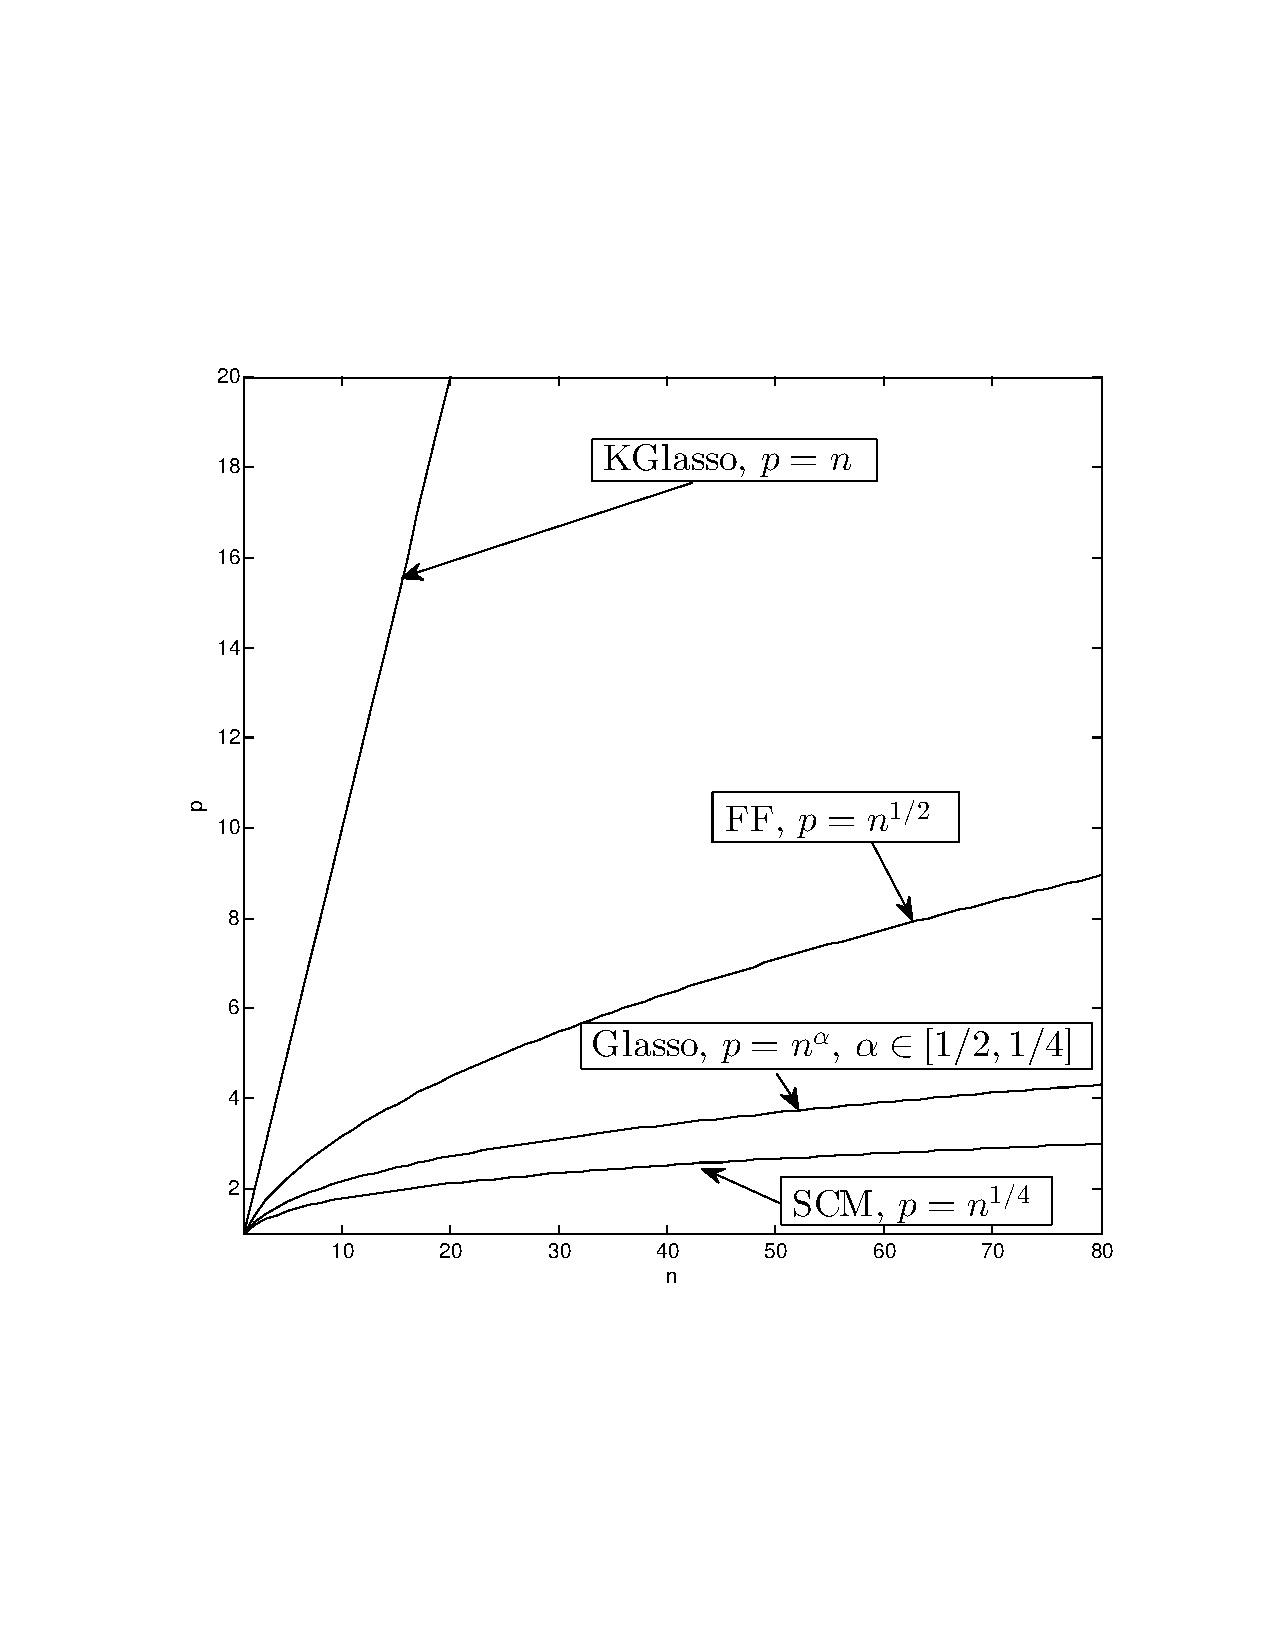
\includegraphics[width=0.50\textwidth]{./Sim/visRates.pdf}
	\caption{Regions of convergence for KGlasso (below upper curve), FF (below second highest curve), Glasso (below third highest curve), and standard sample covariance matrix estimator (SCM) (bottom curve). These regions are obtained from the analytical expressions in equations (\ref{KGL_perfect_rate}),  (\ref{FF_rate_2}), (\ref{Glasso_rate})  and  (\ref{naive_SCM_rate}), respectively. The simulation shown in Fig. \ref{fig: KGlasso_FF_div_conv} establishes that the FF algorithm indeed diverges when the parameters $p$ and $n$ fall inbetween the KGlasso and FF curves in the above figure.}
	\label{fig: visRate}
\end{figure}

Although Thm. \ref{thm: KGL_optimal_rate} shows a rate on the inverse covariance matrix, this asymptotic rate can be shown to hold for the covariance matrix as well (see proof of Thm. \ref{thm: KGL_optimal_rate} in Appendix).


\subsection{Discussion}
Theorem \ref{thm: KGL_optimal_rate} is established using the large deviation bound in Lemma \ref{lemma: large_dev_Ted}. We provide some intuition on this bound below.
Assume that $\bX_{init} = \bX_0$, or $\bA_{init}=\bX_{init}^{-1}=\bA_0$. Define $\bW= \bX_0^{1/2} \otimes \bI_p$ and $\tilde{\bz}_t = \bW \bz_t$, with i.i.d. $\bz_t\sim N(\mathbf{0}, \bA_0\otimes \bB_0)$, $t=1,\dots,n$. Then, $\tilde{\bz}_t$ has block-diagonal covariance
\begin{equation*}
	\Cov(\tilde{\bz}_t) = \bI_p \otimes \bB_0.
\end{equation*}
When $\bW$ is applied to the transformed $pf\times pf$ sample covariance matrix, $\hat{\bS}_n^W := \bW \hat{\bS}_n \bW^T$, the first step of KGlasso produces an iterate $\hat{\bY}_n^{(1)}=\bG(\hat{\bB},\lambda_Y)$ with $\hat{\bB} = \frac{1}{p}\sum_{i=1}^p \hat{\bS}_n^W(i,i)$ (recall (\ref{B_update})). For suitable $\lambda_Y = \lambda_Y^{(1)}$, $\hat{\bY}_n^{(1)}$ converges to $\bY_0$ with respect to maximal elementwise norm at a rate $O_P\left( \sqrt{\frac{\log M}{np}} \right)$. The convergence of $\hat{\bY}_n^{(1)}$ is easily established by applying the Chernoff bound and invoking the jointly Gaussian property of the measurements and the block diagonal structure of $\Cov(\tilde{\bz}_t)$. Lemma \ref{lemma: large_dev_Ted} in the Appendix establishes that this rate holds even if $\bX_{init}\neq \bX_0$ in Assumption \ref{assumption_posdef_unif}. In view of the rate of convergence of $\hat{\bY}^{(1)}$, to achieve a reduction in the MSE of $\bY$, either the sample size $n$ or the dimension $p$ must increase. Lemma \ref{lemma: large_dev_Ted} provides a tight bound that makes the dependence of the convergence rate explicit in $p,f$ and $n$. Theorem \ref{thm: KGL_optimal_rate} uses Lemma \ref{lemma: large_dev_Ted} to show that KGlasso converges to $\bX_0\otimes \bY_0$ with rate $O_P\left( \sqrt{\frac{(p+f)\log M}{n}} \right)$ with respect to Frobenius norm.



\section{Simulation Results} \label{sec: simulations}

In this section, we empirically validate the convergence rates established in previous sections using Monte Carlo simulation. 

Each iteration of the KGlasso involves solving an $\ell_1$ penalized covariance estimation problem of dimension $100 \times 100$ (Step 6 and Step 8 of KGlasso specified by Algorithm \ref{alg: algKGL}). To solve these small sparse covariance estimation problems we used the Glasso algorithm of Hsieh {\it et al} \cite{HsiehNIPS11} where the Glasso stopping criterion was determined by monitoring when the duality gap falls below a threshold of $10^{-3}$.

In each of the simulations the true covariance matrix factors  $\bX_0=\bA_0^{-1}$ and $\bY_0=\bB_0^{-1}$ were unstructured randomly generated positive definite matrices. First, $p$ random nonzero elements were placed on the diagonal of a square $p \times p$ matrix $C$. Then, on average $p$ nonzero elements were placed on the off-diagonal and symmetry was imposed. On average, a total of $3p$ elements were nonzero. The resulting matrix $\tilde{\bC}$ was regularized to produce the sparse positive definite inverse covariance $\bY_0 = \tilde{\bC} + \rho \bI_f$, where $\rho = 0.5-\lambda_{min}(\tilde{\bC})$. A total of $N_{MC}=50$ simulation runs were performed for each sample size $n$, where $n$ ranged from 10 to 100. Performance assessment was based on normalized Frobenius norm error in the covariance and precision matrix estimates. The normalized error was calculated using
\begin{equation*}
	\sqrt{ \frac{1}{N_{MC}} \sum_{i=1}^{N_{MC}}{ \frac{\nn \bSigma_{0}-\hat{\bSigma}(i) \nn_F^2}{\nn \bSigma_0 \nn_F^2} } }
\end{equation*}
where $\hat{\bSigma}(i)$ is the covariance estimate for the $i$-th simulation. The same formula was  used to calculate the normalized error in the precision matrix $\hat{\bTheta}_0$.
In the implementation of KGlasso, the regularization parameters were chosen as follows. The initialization was $\bX_{init}=\bI_p$. The regularization parameters were selected as $\lambda_Y^{(1)}= c_y \sqrt{\frac{\log M}{np}}$, $\lambda_X^{(2)}= c_x \sqrt{\frac{\log M}{nf}} + \lambda_Y^{(1)}$, $\lambda_Y^{(2)} = \lambda_X^{(2)}$, $\lambda_X^{(3)}= \lambda_X^{(2)}$ and so on. We set $c_x=c_y=0.4$.

We considered the setting where $\bX_0$ and $\bY_0$ are large sparse matrices of dimension $p=f=100$ (see Fig. \ref{fig: sim4_matrices}) yeilding a covariance matrix $\bTheta_0$ of dimension $10,000 \times 10,000$. This dimension was too large for implementation of Glasso even when implemented using the state-of-the-art algorithm by Hsieh {\it et al} \cite{HsiehNIPS11}. Figures \ref{fig: sim4_frob_inv} and \ref{fig: sim4_frob_cov} compare the root-mean squared error (RMSE) performance in precision and covariance matrices as a function of $n$. As expected, KGlasso outperforms FF over the range of $n$ for both covariance and inverse covariance estimation problems. KGlasso outperforms FF in the small-sample regime since it exploits sparsity in addition to Kronecker structure.

For $n=10$, there is a $72 \%$ ($\approx 5.53$ dB) RMSE reduction for the precision matrix and $49 \%$ RMSE reduction for the covariance matrix when using KGlasso instead of FF. For $n=100$, there is a $51 \%$ ($\approx 3.10$ dB) RMSE reduction for the precision matrix and $41 \%$ RMSE reduction for the covariance matrix. For the small sample regime, there is approximately a $5.53$ dB reduction for the precision matrix, which is a significant performance gain.
\begin{figure}[htp]
	\centering
%		\includegraphics[width=0.40\textwidth]{./Simulations/KGL_FF_sim_21-Mar-2012-22-15_matrices.png}
		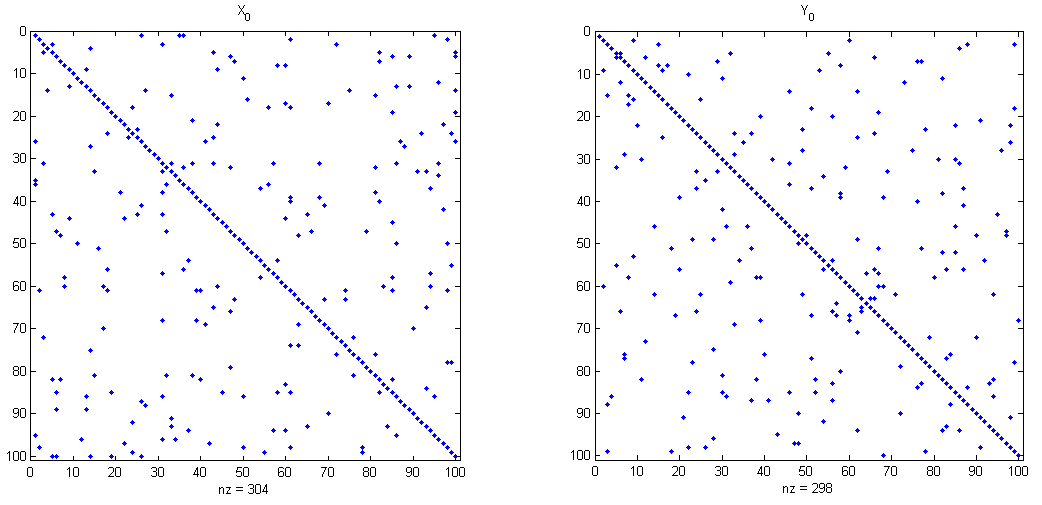
\includegraphics[width=0.40\textwidth]{./Sim/pf100matrices.png}
	\caption{Sparse Kronecker matrix representation. Left panel: left Kronecker factor. Right panel: right Kronecker factor. As the Kronecker-product covariance matrix is of dimension $10,000 \times 10,000$ standard Glasso is not practically implementable for this example.}
	\label{fig: sim4_matrices}
	\vfill
		 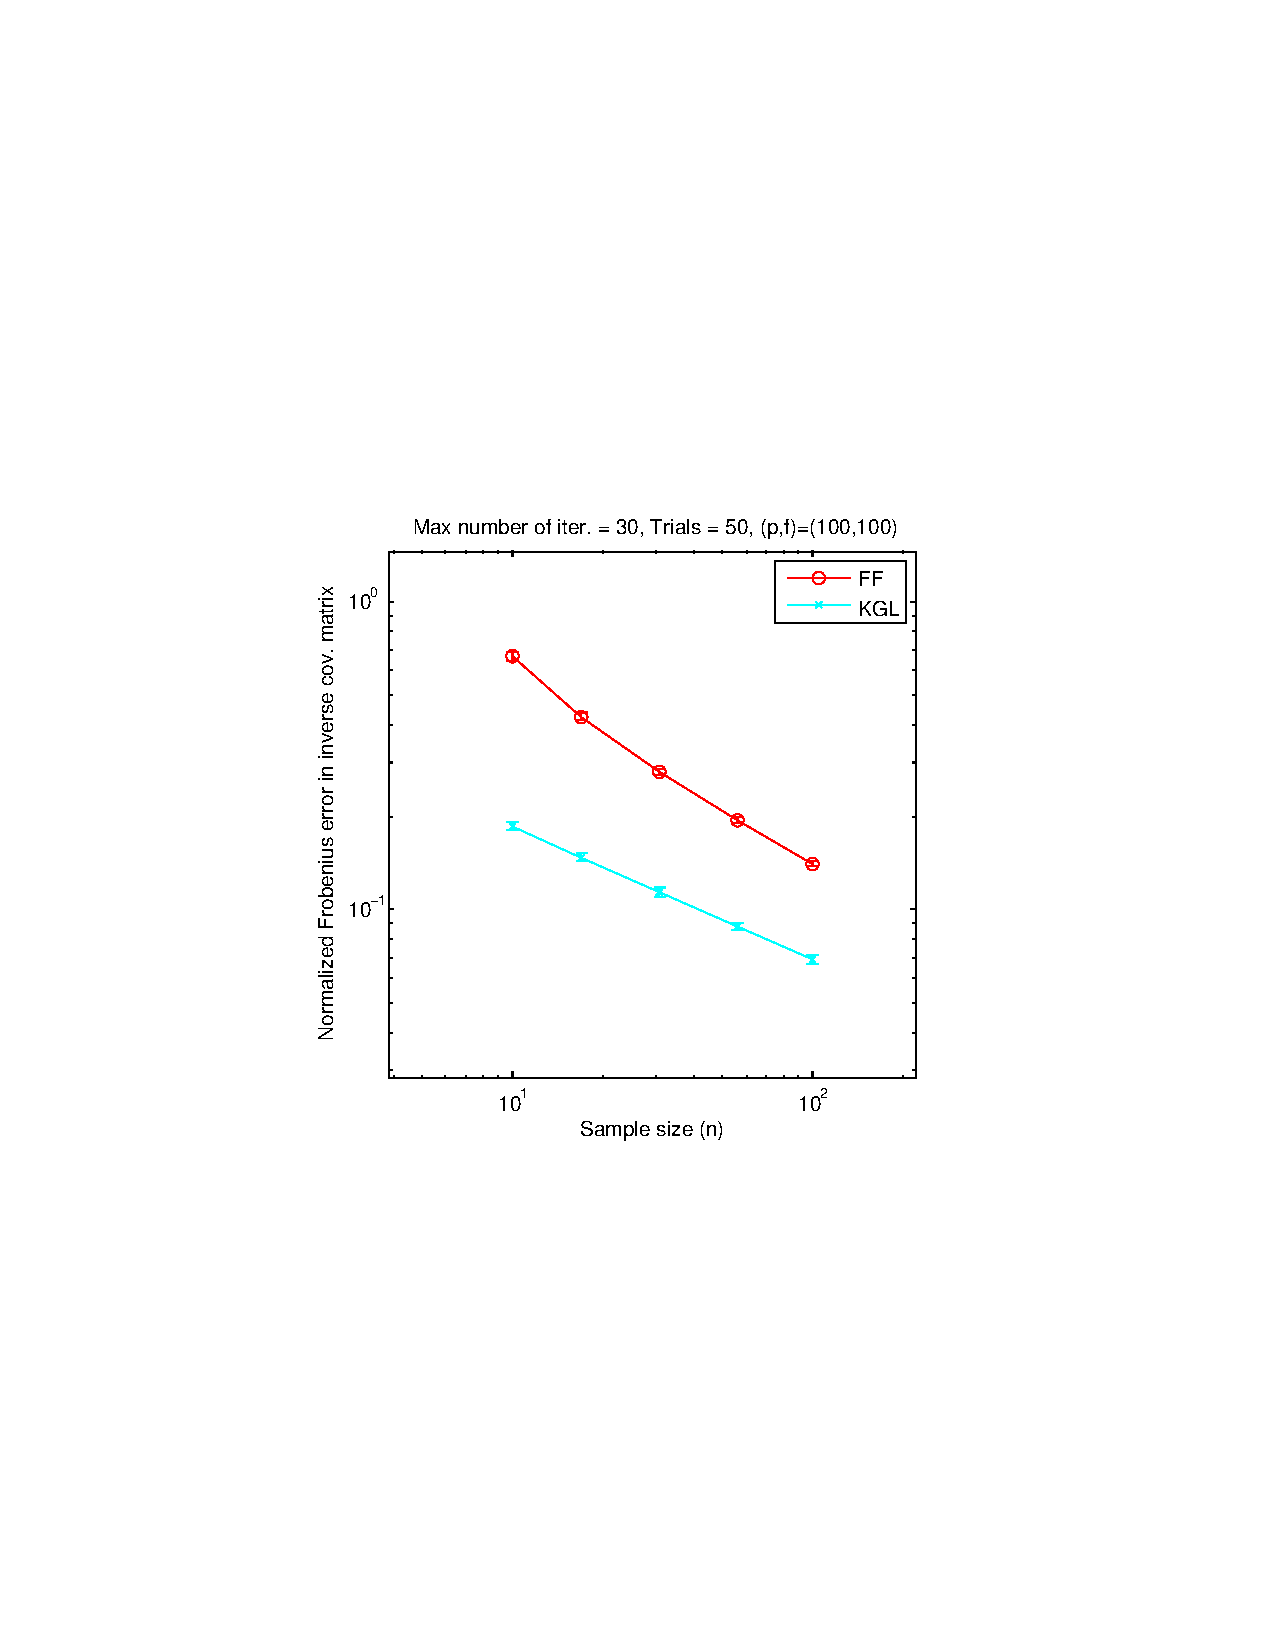
\includegraphics[width=0.40\textwidth]{./Sim/KGL_FF_sim_21-Mar-2012-22-15_Frob_inv_std_all.pdf}
	\caption{Normalized RMSE performance for precision matrix as a function of sample size $n$. KGlasso (Kronecker graphical lasso) uniformly outperforms FF (flip-flop) algorithm for all $n$. Here, $p=f=100$ and $N_{MC}=50$. The error bars are centered around the mean with $\pm$ one standard deviation. For $n=10$, there is a $72 \%$ RMSE reduction.  }
	\label{fig: sim4_frob_inv}
	\vfill
		 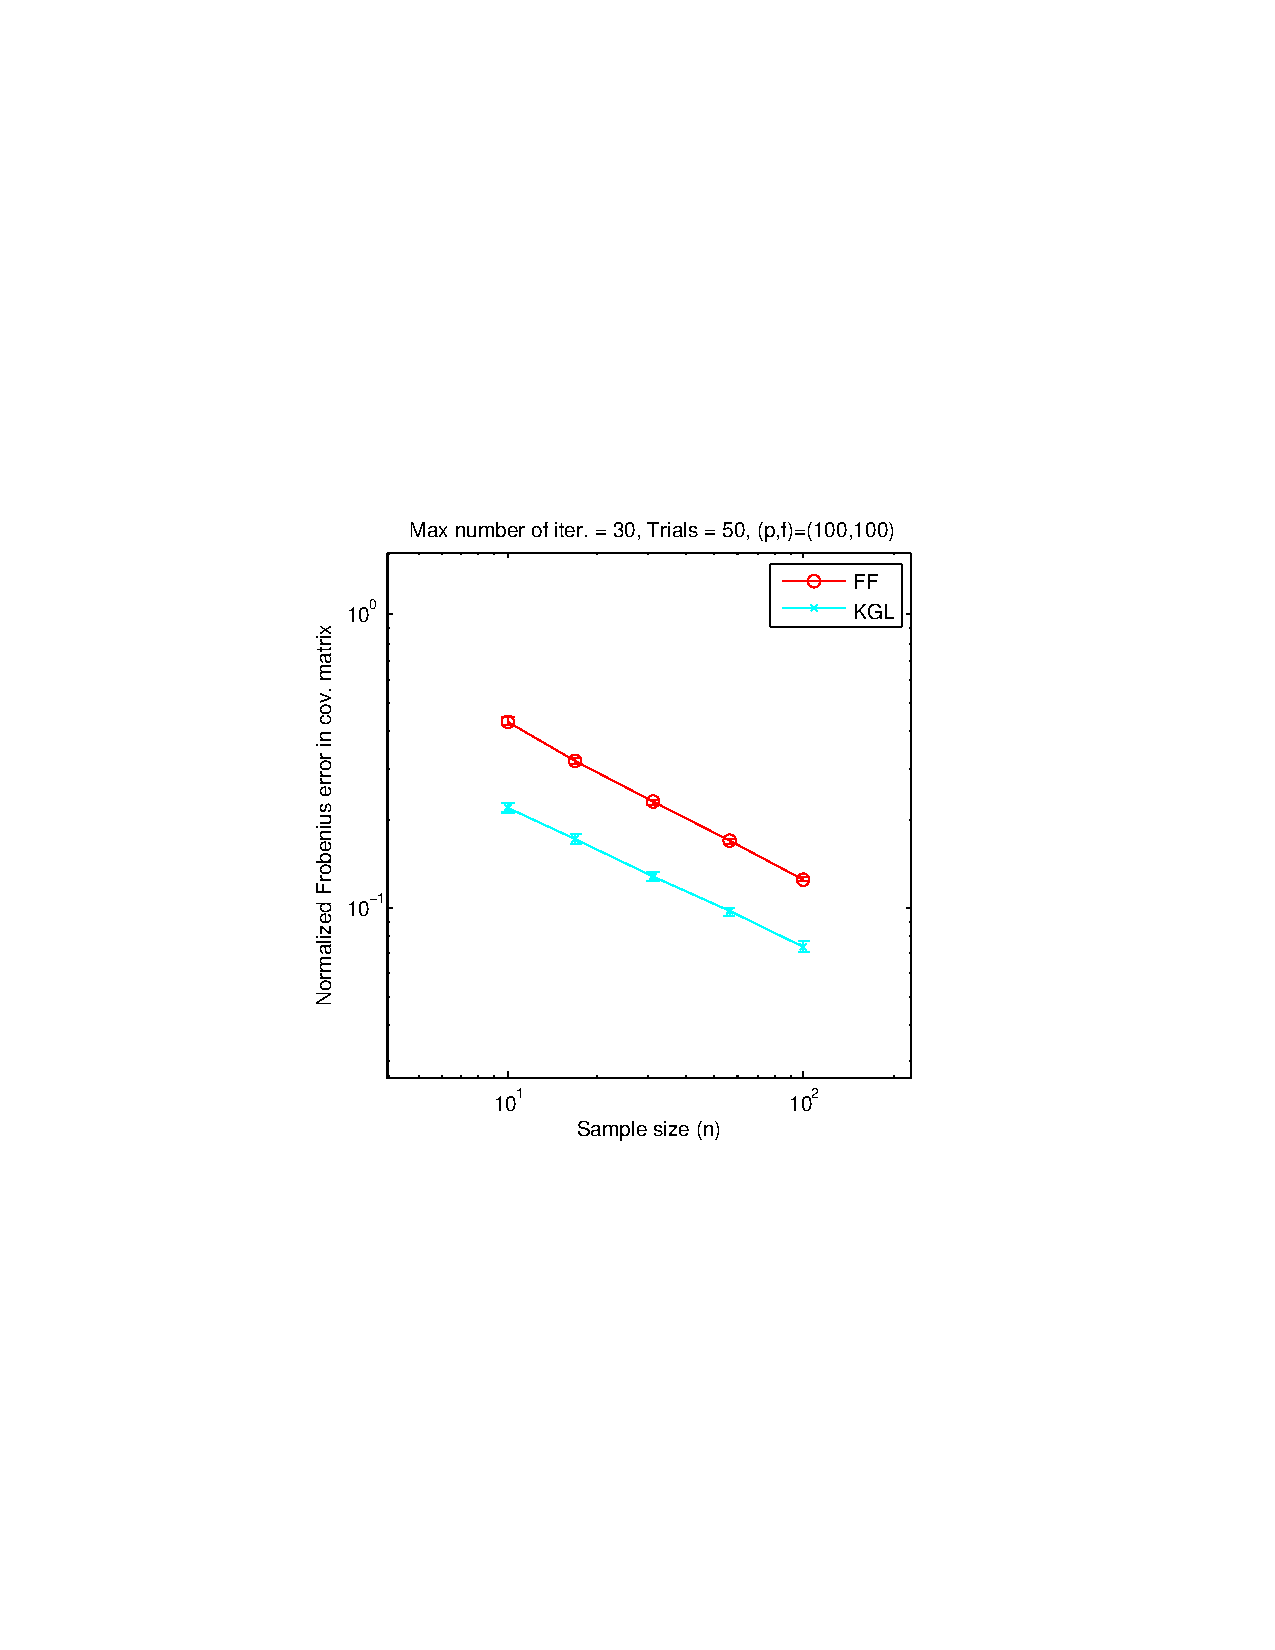
\includegraphics[width=0.40\textwidth]{./Sim/KGL_FF_sim_21-Mar-2012-22-15_Frob_cov_std_all.pdf}
	\caption{Normalized RMSE performance for covariance matrix as a function of sample size $n$. KGlasso (Kronecker graphical lasso) uniformly outperforms FF (flip-flop) algorithm for all $n$. Here, $p=f=100$ and $N_{MC}=50$. The error bars are centered around the mean with $\pm$ one standard deviation. For $n=10$, there is a $49 \%$ RMSE reduction. }
	\label{fig: sim4_frob_cov}
\end{figure}


\subsection{Empirical Rate Comparison}
Next, we illustrate the rates obtained in for the dimension setting $p(n)=f(n)= \lceil 8 n^\alpha \rceil$, where $\alpha\in\{0.1,0.2,0.3\}$. According to the theory developed, for large $n$, the MSE converges to zero at a certain convergence rate. The predicted rates of FF and KGlasso are fitted on top of the empirical MSE curves by ensuring intersection at $n=1000$. Fig. \ref{fig: KGlasso_FF_curves} shows that the empirical rates match the predicted rates well.
\begin{figure}[htp]
	\centering
		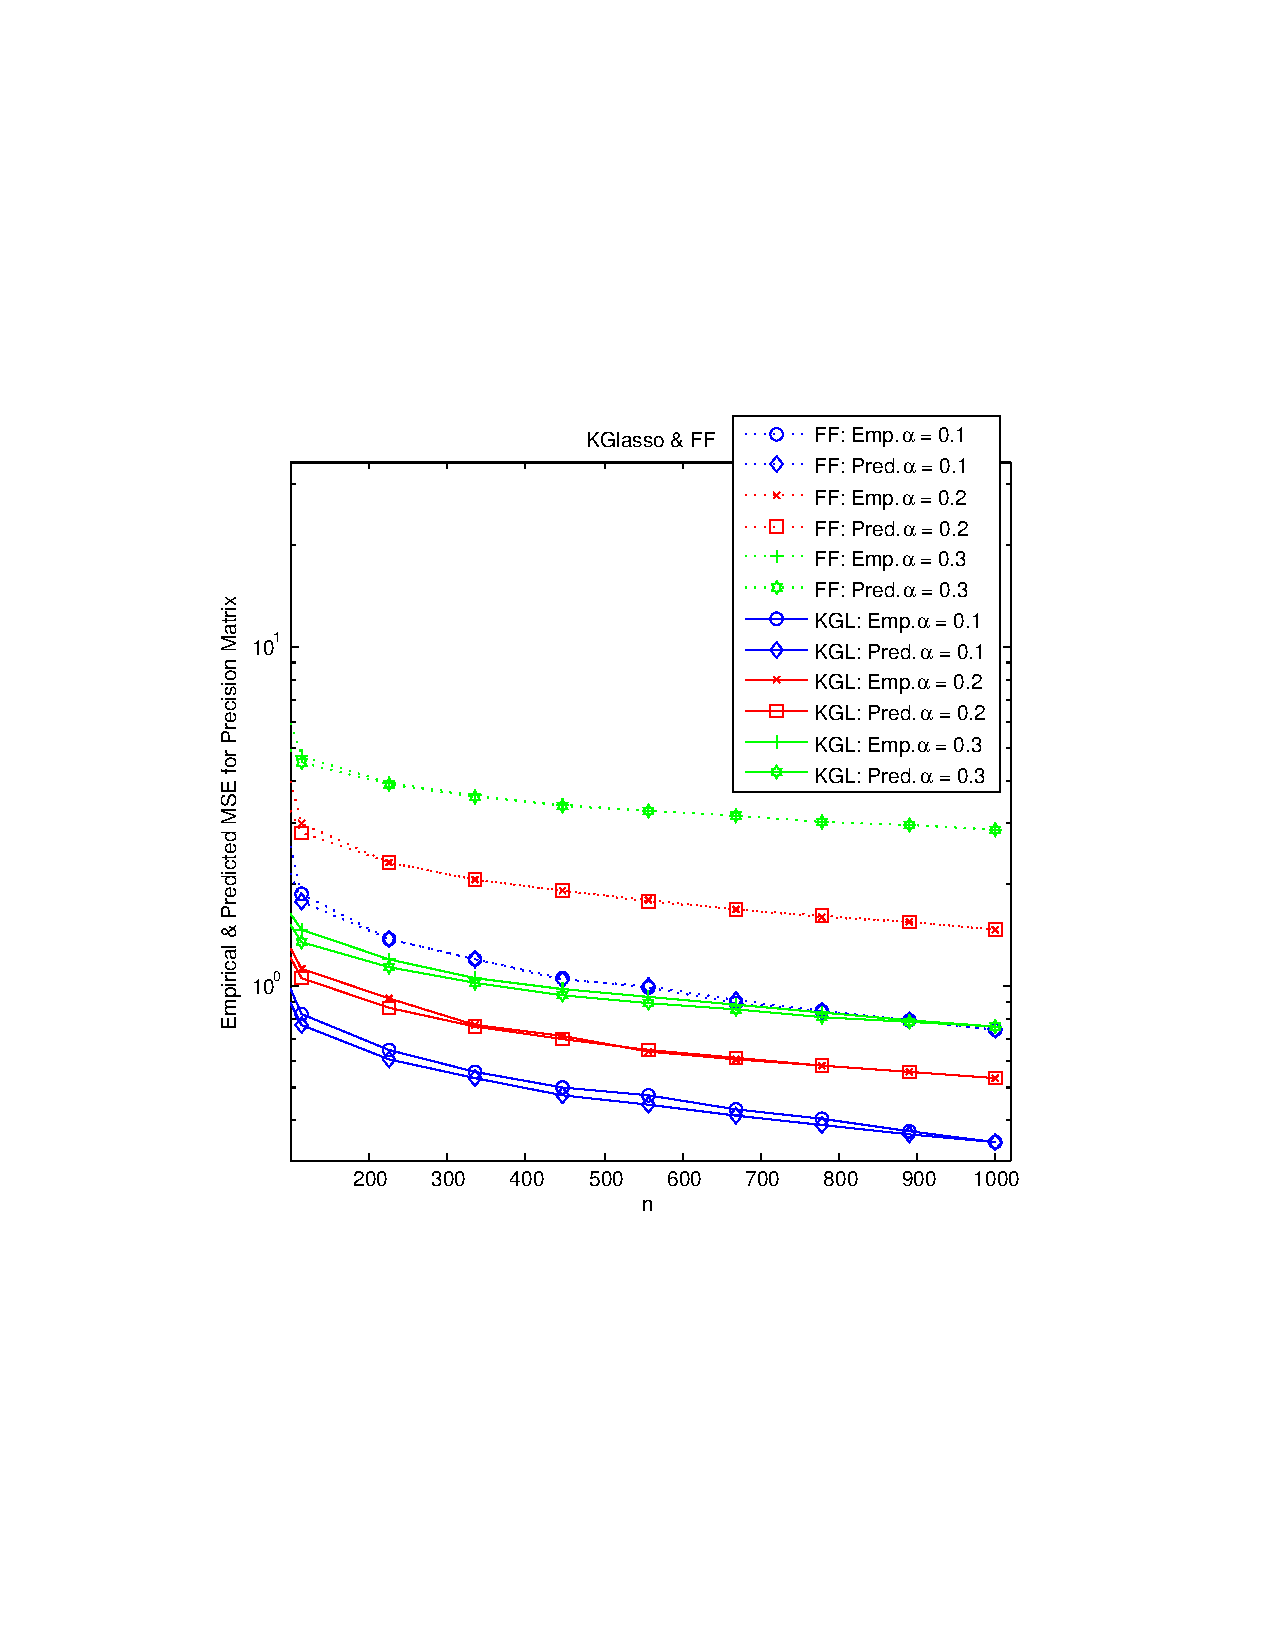
\includegraphics[width=0.50\textwidth]{./Sim/KGlasso_FF_sim_19-Mar-2012-20-19_summary.pdf}
	\caption{ Precision Matrix MSE convergence as a function of sample size $n$ for FF and KGlasso. The dimensions of the Kronecker factor matrices grow as a function of $n$ as: $p(n)=f(n)=\lceil 8 \cdot n^\alpha \rceil$. The true Kronecker factors were set to identity (so their inverses are fully sparse). The predicted MSE curves according to Thm. \ref{thm: FF_optimal_rate} and Thm. \ref{thm: KGL_optimal_rate} are also shown. For both KGlasso and FF, the predicted MSE matches the empirical MSE well, thus verifying the rate expressions (\ref{FF_rate_2}) and (\ref{KGL_perfect_rate}). }
	\label{fig: KGlasso_FF_curves}
\end{figure}

We also show a borderline case $p=f=\lceil n^{0.6} \rceil$. In this case, according to Thm. \ref{thm: FF_optimal_rate} and Thm. \ref{thm: KGL_optimal_rate}, the FF diverges (MSE increases in $n$), while the KGlasso converges (MSE decreases in $n$). This is illustrated in Fig. \ref{fig: KGlasso_FF_div_conv}. Our predicted rates are plotted on top of the empirical curves.
\begin{figure}[htp]
	\centering
		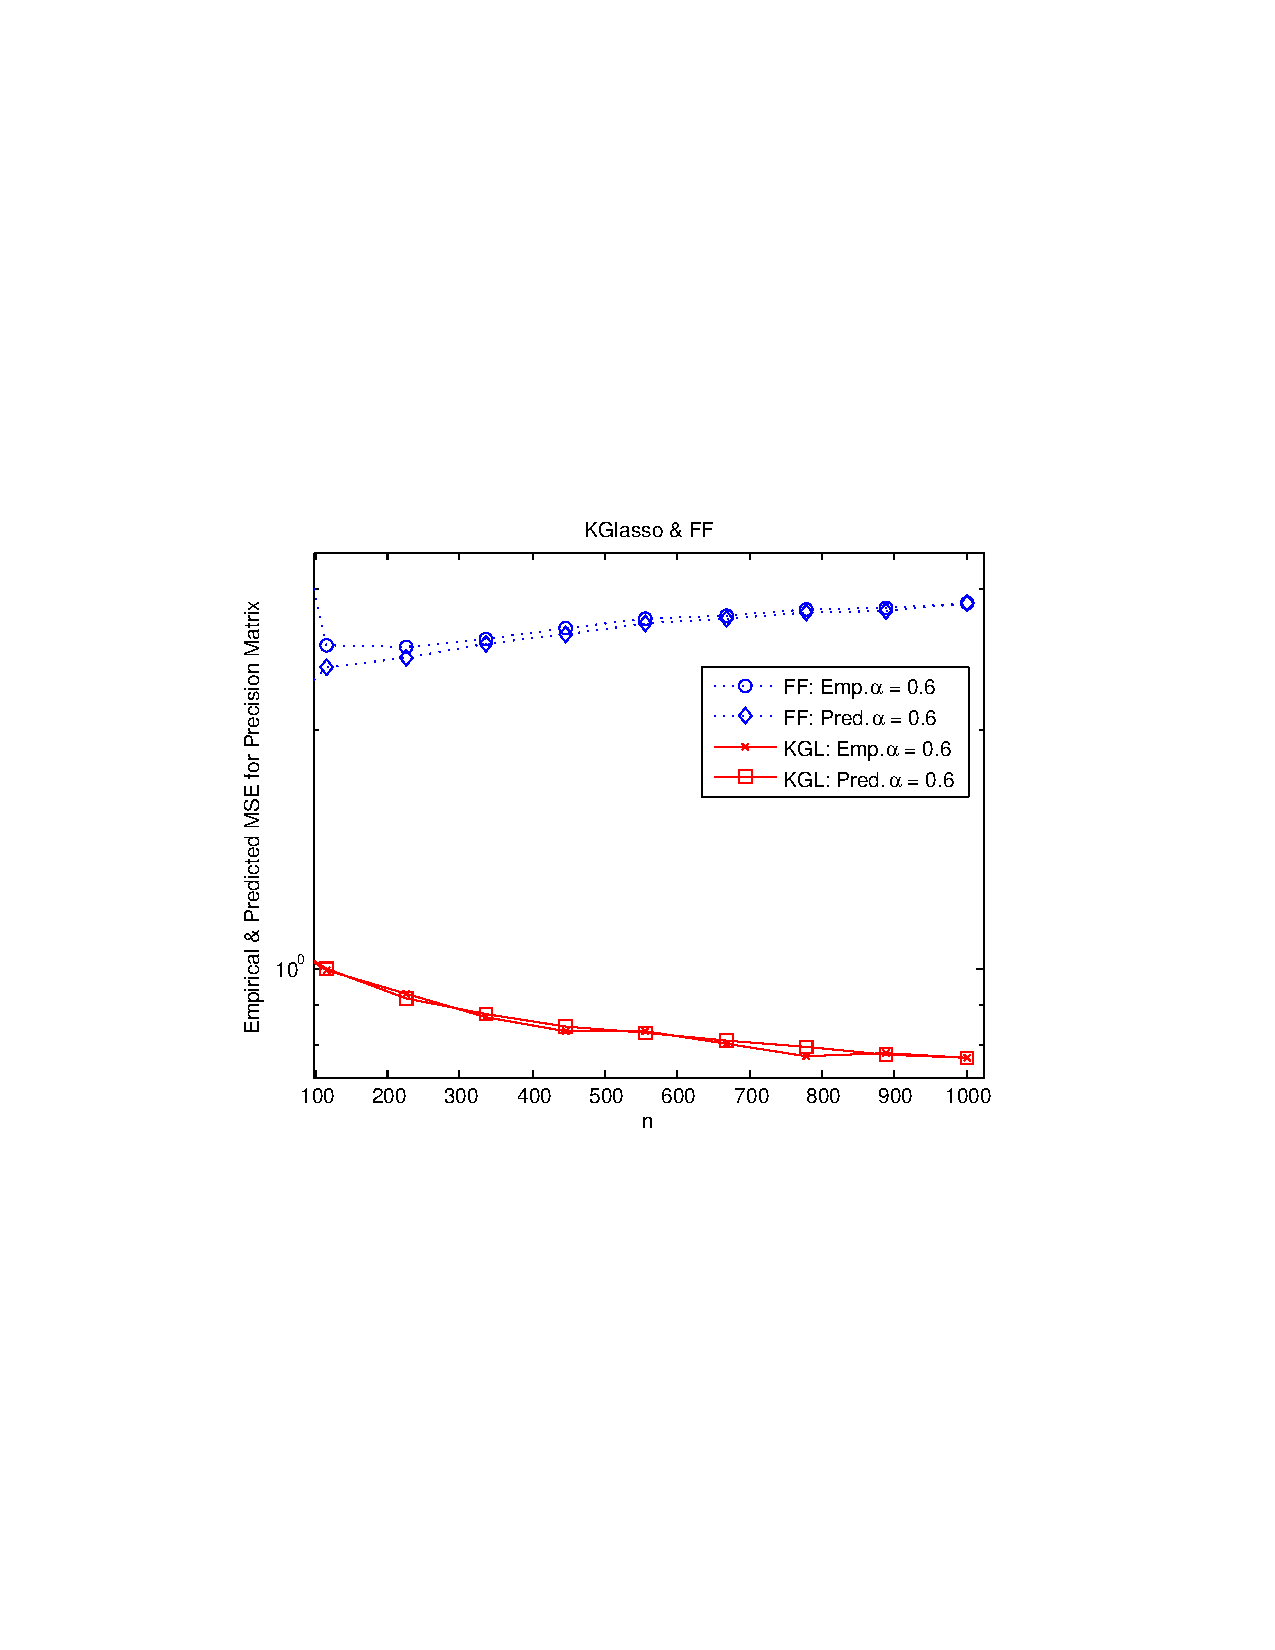
\includegraphics[width=0.50\textwidth]{./Sim/KGlasso_FF_sim_20-Mar-2012-22-54_inv_KGL_FF_pred.pdf}
	\caption{ Precision Matrix MSE as a function of sample size $n$ for FF and KGlasso. The dimensions of the Kronecker factor matrices grow as a function of $n$ as: $p(n)=f(n)=\lceil n^{0.6} \rceil$. The true Kronecker factors were set to identity (so their inverses are fully sparse). The predicted MSE curves according to Thm. \ref{thm: FF_optimal_rate} and Thm. \ref{thm: KGL_optimal_rate} are also shown. As predicted by our theory, and by the predicted convergent regions of $(n,p)$ for FF and KGlasso in Fig. \ref{fig: visRate},  the MSE of the FF diverges while the MSE of the KGlasso converges as $n$ increases. }
	\label{fig: KGlasso_FF_div_conv}
\end{figure}




\section{Conclusion}
We established high dimensional consistency for Kronecker Glasso algorithms that use iterative $\ell_1$-penalized likelihood optimization that exploit both Kronecker structure and sparsity of the covariance. A tight MSE convergence rate was derived for KGlasso, showing significantly better MSE performance than standard Glasso \cite{Rothman, ModelSel} and FF \cite{EstCovMatKron}. Simulations validated our theoretical predictions. 


\section*{Acknowledgement}
The authors thank Prof. Mark Rudelson for very helpful discussions on large deviation theory.


% Appendices with technical proofs
\appendices

\section{Proof of Lemma \ref{dual_lemma}}
\begin{IEEEproof}
\begin{enumerate}
	\item Without loss of generality, fix $\bY\in S_{++}^f$. The function $\tr((\bX \otimes \bY)\hat{\bS}_n)$ is linear in $\bX$.	The function $g(\mathbf{X}_1):=-\log\det(\mathbf{X}_1)$ is a convex function in $\mathbf{X}_1$ over the set $S_{++}^p$ \cite{ConvexOpt}. The triangle inequality implies $|\cdot|_1$ is convex. Finally, the sum of convex functions is convex.	The set $S_{++}^p$ is a convex set for any $p\in \mathbb{N}$.
	\item By symmetry we only need prove that (\ref{dualX}) is the dual of $\min_{\mathbf{Y}\in S_{++}^f} J_\lambda(\bX,\bY)$. By standard duality relations between $\ell_1$ and $\ell_\infty$ norms \cite{ConvexOpt} and symmetry of $\bY$ \footnote{ The maximum is attained at $\mathbf{U}_{i,j}= \frac{\mathbf{Y}_{i,j}}{|\mathbf{Y}_{i,j}|}$ for $\mathbf{Y}_{i,j}\neq 0$ and at $\mathbf{U}_{i,j}=0$ for $\mathbf{Y}_{i,j}=0$.}: 
	\begin{equation*}
		|\mathbf{Y}|_1=\max_{\mathbf{U}\in S^f: |\mathbf{U}|_{\infty}\leq 1}{\tr(\mathbf{Y}\mathbf{U})}
	\end{equation*}
	Using this in (\ref{J_lambda_func}) and invoking the saddlepoint inequality:
	\begin{align}
	  &\min_{\mathbf{Y}\in S_{++}^f}  {\tr((\mathbf{X}\otimes \mathbf{Y})\hat{\bS}_n)-p\log\det(\mathbf{Y})+p\lambda_Y |\bY|_1} \nonumber \\
	  	%&= \min_{\mathbf{Y}\in S_{++}^f} \max_{|\mathbf{U}|_{\infty}\leq \lambda_Y} \Big\{ \tr((\mathbf{X}\otimes \mathbf{Y})\hat{\bS}_n)-p\log\det(\mathbf{Y})\nonumber \\
	  	%& \qquad +p \tr(\mathbf{Y}\mathbf{U}) \Big\} \nonumber \\
	    &\geq \max_{|\mathbf{U}|_{\infty}\leq \lambda_Y} \min_{\mathbf{Y}\in S_{++}^f} \Big\{ \tr((\mathbf{X}\otimes \mathbf{Y})\hat{\bS}_n)-p\log\det(\mathbf{Y}) \nonumber \\
	    & \qquad +p \tr(\mathbf{Y}\mathbf{U}) \Big\} \label{saddle_ptY}
	\end{align}
When the equality in (\ref{saddle_ptY}) is achieved, $(\bU,\mathbf{Y})$ is a saddlepoint and the duality gap is zero. Rewrite the objective function, denoted $\tilde{J}_\lambda(\cdot,\cdot)$, in the minimax operation (\ref{saddle_ptY}):
	\begin{equation*}
		\tilde{J}_\lambda(\bX,\bY):= \tr((\bX\otimes \bY)(\hat{\bS}_n+\tilde{\bU}(\bX)))-p\log\det(\bY)
	\end{equation*}
	where $\tilde{\mathbf{U}}(\mathbf{X})=p \frac{\bI_p \otimes \bU}{\tr(\bX)}$. Define $\bM=\hat{\bS}_n + \tilde{\bU}(\bX)$. To evaluate $\min_{\bY \in S_{++}^f}{\tilde{J}_\lambda(\bX,\bY)}$ in (\ref{saddle_ptY}), we invoke the KKT conditions to obtain the solution $\bY=\left( \frac{1}{p} \sum_{i,j=1}^p{\bX_{i,j} \bM(j,i))} \right)^{-1}$. Define $\bW=\bY^{-1}$ as the dual space variable. Using this in (\ref{saddle_ptY}):
	\begin{equation} \label{dualY_full}
		\max_{|\bW-\frac{1}{p}\sum_{i,j=1}^p{\bX_{i,j} \hat{\bS}_n(j,i)}|_{\infty}\leq \lambda_Y } p \log\det(\mathbf{W}) + pf
	\end{equation}
	where the constraint set was obtained in terms of $\bW$ by observing that $\tilde{\mathbf{U}}(\mathbf{X})(j,i) = \frac{p \mathbf{U}}{\tr(\mathbf{X})} I(j=i)$, and $I(\cdot)$ is the indicator function. 
%	Note that a cancellation occured in (\ref{dualY_full}) which is due to the identity:
%	\begin{align}
%		\tr&((\mathbf{X}\otimes \mathbf{Y})\mathbf{M}) = \sum_{i=1}^p{ \tr \left( \sum_{j=1}^p{ \mathbf{X}_{i,j} \mathbf{Y} \mathbf{M}(j,i) } \right) } \nonumber \\
%			%&=  \tr \left( \sum_{i=1}^p{  \sum_{j=1}^p{ \mathbf{X}_{i,j} \mathbf{M}(j,i) \mathbf{Y} } } \right) \nonumber \\
%			&=  p \tr \left( \sum_{i=1}^p { \sum_{j=1}^p{ \mathbf{X}_{i,j} \mathbf{M}(j,i)} \Big( \sum_{i,j=1}^p{ \mathbf{X}_{i,j} \mathbf{M}(j,i) \Big)^{-1}} } \right) \nonumber \\
%			&=  pf \nonumber
%	\end{align}
%	where $\mathbf{M}(j,i)$ denotes the $(j,i)$th $f\times f$ sub-block of the $pf\times pf$ symmetric matrix $\mathbf{M}$.
	It is evident that (\ref{dualY_full}) is equivalent to (\ref{dualY}).

	\item It suffices to verify that the duality induced by the saddle point formulation is equivalent to Lagrangian duality (see Section 5.4 in \cite{ConvexOpt}). Slater's constraint qualification (see Section 5.3.2 in \cite{ConvexOpt}) trivially holds for the convex problem $\min_{\mathbf{Y} \in S_{++}^f}\tilde{J}_\lambda(\mathbf{X},\mathbf{Y})$, and thus for the corresponding convex problem $\min_{\mathbf{Y} \in S_{++}^f}J_\lambda(\mathbf{X},\mathbf{Y})$. Since the objective function of each dual problem has an optimal objective that is bounded below, Slater's constraint qualification also implies that the dual optimal solution is attained.

	\item From \cite{EstCovMatKron}, it follows that if $\hat{\bS}_n$ is p.d., each ``compression step'' (see lines 6 and 8 in Algorithm \ref{alg: algKGL}) yields a p.d. matrix. Combining this with the positive definiteness of the Glasso estimator \cite{ModelSel}, we conclude that the first subiteration of KGlasso yields a p.d. matrix. A simple induction, combined with the fact that the Kronecker product of p.d. matrices is p.d., establishes that (\ref{dualY}) and (\ref{dualX}) are p.d.

\end{enumerate}
	
	
	
\end{IEEEproof}


%\section{Limit Point Characterization of KGlasso}
%%MOVE THIS ENTIRE SECTION (TO POINT A) TO THE APPENDIX
%%We first show that the KGlasso iterations converge to a fixed point.
%Let $J_\lambda(\bX,\bY)$ be as defined in (\ref{J_lambda_func}) and define $J_\lambda^{(k)}=J_\lambda(\mathbf{X}^{(k)},\mathbf{Y}^{(k)})$ for $k=0,1,2,\dots$.
%
%\begin{theorem} \label{convergence_fixed_point}
%	If $\hat{\bS}_n$ is positive definite, the KGlasso iterations converge to a fixed point. Also, we have $J_\lambda^{(k)} \searrow J_\lambda^{(\infty)}$.
%\end{theorem}
%\begin{IEEEproof}
%	Recall that the basic optimization problem (\ref{opt_prob}) is
%	\begin{equation*}
%		\min_{\bX \in S_{++}^p, \bY \in S_{++}^f} J_\lambda(\bX,\bY)
%	\end{equation*}
%	Let $J^*:=\inf_{\mathbf{X} \in S_{++}^p, \mathbf{Y} \in S_{++}^f}{J_\lambda(\mathbf{X},\mathbf{Y})}$ be the optimal primal value. Note that $J_\lambda^* > -\infty$ when $\hat{\bS}_n \in S_{++}^{pf}$. Consider Algorithm \ref{alg: algKGL}. Assuming $\bX^{(0)}$ and $\hat{\bS}_n$ are p.d., Lemma \ref{dual_lemma} implies that all the iterates are p.d. and
%	\begin{equation} \label{monotonicity}
%		J_\lambda(\bX^{(k)},\bY^{(k)}) \leq	J_\lambda(\bX^{(k-1)},\bY^{(k)}) \leq J_\lambda(\bX^{(k-1)},\bY^{(k-1)})
%	\end{equation}
%	By induction on the number of iterations, we conclude that the iterates yield a nonincreasing sequence of objective functions. Since $\bar{\lambda}_X |\bX|_1, \bar{\lambda}_Y |\bY|_1 \geq 0$, the maximum likelihood objective function provides a lower bound to the optimal primal value
%	\begin{equation} \label{LB_ML}
%		J_\lambda(\bX^{(k)},\bY^{(k)}) \geq J_\lambda^* \geq J_\lambda(\bX_{ML},\bY_{ML}) > -\infty
%	\end{equation}
%	Thus, the sequence $\{J_\lambda^{(k)}:k\geq 0\}$ forms a nonincreasing sequence bounded below \footnote{This follows since for $n>pf$, the log-likelihood function is bounded above by the log-likelihood evaluated at the sample mean and sample covariance matrix.}. The monotone convergence theorem for sequences \cite{IntroRealAnalysis} implies that $\{J_\lambda^{(k)}\}$ converges monotonically to $J_\lambda^{(\infty)}=\inf_k{J_\lambda^{(k)}}$. By the alternating minimization, we conclude that the sequence of iterates $\{(\mathbf{X}^{(k)},\mathbf{Y}^{(k)})\}_k$ converges since the minimizer at each Glasso step is unique.
%\end{IEEEproof}
%
%
%%The following analysis uses Theorem \ref{convergence_fixed_point} to prove convergence of the KGlasso algorithm to a local minimum. To do this, we consider a more general setting. The KGlasso algorithm is a special case of the block-coordinate descent algorithm. Assuming a $k$-fold Kronecker product structure for the covariance matrix, the optimization problem (\ref{J_lambda_func}) can be written as:
%%\begin{equation} \label{obj_func_matrix}
%%	J_\lambda(\bX_1,\dots,\bX_k) = J_0(\bX_1,\dots,\bX_k) + \sum_{i=1}^k{J_i(\bX_i) + \bar{\lambda}_i \eta_1(\bX_i)}
%%\end{equation}
%%where $\bar{\lambda}_i=\lambda_i/d_i$, $\bX_i \in S_{++}^{d_i}$, $\eta_1(\bX_i):=|\bX_i|_1$, $J_0(\bX_1,\dots,\bX_k):=\tr((\bX_1\otimes \bX_2 \otimes \dots \otimes \bX_k)\hat{\bS}_n)$ and $J_i(\bX_i) = - \prod_{i' \neq i}{d_{i'}} \cdot \log\det(\bX_i)$ for $i=1,\dots,k$.
%%
%%Without loss of generality, by reshaping matrices into appropriate vectors, (\ref{obj_func_matrix}) can be rewritten as:
%%\begin{equation} \label{general_f}
%%	J_\lambda(\mathbf{x}_1,\dots,\mathbf{x}_k) = J_0(\mathbf{x}_1,\dots,\mathbf{x}_k) + \sum_{i=1}^k{J_i(\mathbf{x}_i)+\bar{\lambda}_i \eta_i(\mathbf{x}_i)}
%%\end{equation}
%%where the optimization variable is $\mathbf{x}:=[\mathbf{x}_1^T, \mathbf{x}_2^T,\dots,\mathbf{x}_k^T]^T \in \RR^{d'}$, where $\mathbf{x}_i\in \RR^{d_i^2}$ and $d'=\sum_{i=1}^k{d_i^2}$. For example, $\eta_i(\mathbf{X}_i)=|\mathbf{X}_i|_1=\nn \vec(\mathbf{X}_i) \nn_1 = \nn \mathbf{x}_i\nn_1 = \eta_i(\mathbf{x}_i)$. The mapping $\{J_i\}_{i=0}^k$ can be similarly written in terms of the vectors $\mathbf{x}_i$ instead of the matrices $\mathbf{X}_i$.
%%
%%
%%The general optimization problem of interest here is:
%%\begin{equation} \label{gen_func}
%%	\min_{\mathbf{x} \in \RR^{d'}} {J_\lambda(\mathbf{x})} \text{ subject to } \vec^{-1}(\mathbf{x}_i)=\bX_i \in S_{++}^{d_i}, i=1,\dots,k
%%\end{equation}
%%The positive definiteness constraints are automatically taken care of by the construction of the algorithm (see Lemma \ref{dual_lemma}.4). Let the dimension of the covariance matrix be denoted by $d:=\prod_{i=1}^k{d_i}$. We assume $n>d$. To solve (\ref{gen_func}), a block coordinate-descent penalized algorithm can be constructed \cite{TsiligkaridisTSP} that iteratively optimizes (\ref{obj_func_matrix}).
%%
%%%\begin{algorithm}
%%%\caption{Block Coordinate-Descent Penalized Algorithm}
%%%\label{alg: alg2}
%%%\begin{algorithmic}[1]
%%%\STATE \textbf{Input:}  {$\hat{\bS}_n$, $d_i$, $n$, $\epsilon>0$, $\lambda_i >0$}
%%%\STATE \textbf{Output:} {$\hat{\bTheta}$}
%%%
%%%	\STATE Initialize $\mathbf{X}_1^0, \mathbf{X}_2^0, \dots, \mathbf{X}_k^0$ matrices as positive definite matrices, e.g., scaled identity.
%%%	
%%%	\STATE $\hat{\mathbf{\Theta}}_0 \leftarrow \mathbf{X}_1^0\otimes \mathbf{X}_2^0 \otimes \dots \otimes \mathbf{X}_k^0$\;
%%%	
%%%	\STATE $m \leftarrow 0$\;
%%%	\REPEAT {
%%%		\STATE $\hat{\mathbf{\Theta}}_{\text{prev}} \leftarrow \hat{\mathbf{\Theta}}$
%%%		
%%%		\STATE $\mathbf{X}_1^m \leftarrow \arg \min_{\mathbf{A}_1 \succ 0} J_\lambda(\mathbf{A}_1,\mathbf{X}_2^{m-1},\dots,\mathbf{X}_k^{m-1})$
%%%		\STATE $\mathbf{X}_2^m \leftarrow \arg \min_{\mathbf{A}_2 \succ 0} J_\lambda(\mathbf{X}_1^m,\mathbf{A}_2,\dots,\mathbf{X}_k^{m-1})$
%%%		\STATE $\vdots$
%%%		\STATE $\mathbf{X}_k^m \leftarrow \arg \min_{\mathbf{A}_k \succ 0} J_\lambda(\mathbf{X}_1^m,\mathbf{X}_2^m,\dots,\mathbf{A}_k)$
%%%		
%%%		\STATE $\hat{\mathbf{\Theta}} \leftarrow \mathbf{X}_1^m \otimes \mathbf{X}_2^m \otimes \dots \otimes \mathbf{X}_k^m$
%%%		
%%%		\STATE $m \leftarrow m + 1$
%%%	}	\UNTIL {$\frac{\nn \hat{\mathbf{\Theta}}_{\text{prev}}-\hat{\mathbf{\Theta}} \nn}{\nn \hat{\bTheta}_{\text{prev}} \nn} \leq \epsilon$}
%%%	
%%%\end{algorithmic}
%%%\end{algorithm}
%%%
%%%\begin{remark}
%%%	The positive definiteness constraint at each coordinate descent iteration of Algorithms \ref{alg: algKGL} and \ref{alg: alg2} need not be explicit since the objective function $J_\lambda(\cdot)$ acts as a logarithmic barrier function.
%%%\end{remark}
%%
%%Note that Algorithm \ref{alg: algKGL} would be a special case of this algorithm. An extension of Theorem \ref{convergence_fixed_point}, assuming $n>d$ or $J_\lambda^*> -\infty$, based on induction, can be used to show that the limit points of the sequence of iterates $(\mathbf{x}^m)_{m\geq 0}=(\mathbf{x}_1^m,\dots,\mathbf{x}_k^m)_{m \geq 0}$ are fixed points.
%
%\begin{remark}
%	Note that a necessary condition for $\mathbf{x}^*$ to minimize $J_\lambda$ is $0\in \partial J_\lambda(\mathbf{x}^*)$. This is not sufficient however.
%\end{remark}
%
%We next show that the limit point(s) of $(\mathbf{x}^m)_{m\geq 0}$ are nonempty and are local minima.
%
%\begin{theorem} \label{convergence_theorem_critical_manyfactors}
%	Let $(\mathbf{x}^m)=(\mathbf{x}_1^m,\dots,\mathbf{x}_k^m)_{m\geq 0}$ be a sequence generated by the block-coordinate descent algorithm. Assume $n>d$.
%
%\begin{enumerate}
%	%\item The KGlasso iterations converge to a local minimum or a local maximum of the objective function.
%	\item The iterates converge to a local minimum or a local maximum of the objective function.
%	\item If the initial condition $\mathbf{x}^0$ is not a local maximum then the algorithm converges to a local minimum.
%\end{enumerate}
%\end{theorem}
%\begin{IEEEproof}
%	Due to limited space, the proof is included in \cite{TsiligkaridisTSP}.
%\end{IEEEproof}
%%\begin{IEEEproof}
%%	Define the set of critical points $C_J:=\{\mathbf{x}: 0\in \partial J(\mathbf{x})\}=C_{J,min} \cup C_{J,saddle} \cup C_{J,max}$, where $C_{J,min}$ contains all the local minima, $C_{J,saddle}$ contains all the saddle points and $C_{J,max}$ contains all the local maxima.
%%	
%%\begin{enumerate}
%%	\item Let $L(\mathbf{x}^0)=L(\mathbf{x}_1^0,\dots,\mathbf{x}_k^0)$ be the set of all limit points of $(\mathbf{x}^m)_{m\geq 0}$ starting from $\mathbf{x}^0$. By joint continuity of the objective, we have $J_\lambda(\mathbf{x}^{m_j}) \to J_\lambda(\mathbf{x}^*)$ as $j\to\infty$.
%%	%By the continuity of $J_i$, we have $\sum_{i=1}^k{J_i(\mathbf{x}_i^{m_j})} \to \sum_{i=1}^k{J_i(\mathbf{x}_i^*)}$ as $j \to \infty$. Since $J_0(\cdot)$ is jointly continuous, $J_0(\mathbf{x}_1^{m_j},\dots,\mathbf{x}_k^{m_j}) \to J_0(\mathbf{x}_1^*,\dots,\mathbf{x}_k^*)$. By continuity of $\eta_i(\cdot)$, $\sum_{i=1}^k{\bar{\lambda}_i \eta_i(\mathbf{x}_i^{m_j})} \to \sum_{i=1}^k \bar{\lambda}_i \eta_i(\mathbf{x}_i^*)$. Thus, $J_\lambda(\mathbf{x}^{m_j}) \to J_\lambda(\mathbf{x}^*)$ as $j\to\infty$.
%%	Note that $\nabla J_0$ is uniformly continuous on bounded subsets of its domain. Define the sequence $\{(x_i^m)^o\}_m$ as
%%	\begin{align*}
%%		(\mathbf{x}_1^m)^\circ & := \nabla_{\mathbf{x}_1}J_0(\mathbf{x}_1^m,\mathbf{x}_2^m\dots,\mathbf{x}_k^m) \\
%%			&\quad - \nabla_{\mathbf{x}_1}J_0(\mathbf{x}_1^m,\mathbf{x}_2^{m-1}\dots,\mathbf{x}_k^{m-1}) \\
%%		(\mathbf{x}_2^m)^\circ & := \nabla_{\mathbf{x}_2}J_0(\mathbf{x}_1^m,\mathbf{x}_2^m\dots,\mathbf{x}_k^m) \\
%%			&\quad - \nabla_{\mathbf{x}_2}J_0(\mathbf{x}_1^m,\mathbf{x}_2^m,\mathbf{x}_{3}^{m-1}\dots,\mathbf{x}_k^{m-1}) \\
%%		&\vdots \\
%%		(\mathbf{x}_j^m)^\circ & := \nabla_{\mathbf{x}_j}J_0(\mathbf{x}_1^m,\mathbf{x}_2^m\dots,\mathbf{x}_k^m) \\
%%			&\quad - \nabla_{\mathbf{x}_j}J_0(\mathbf{x}_1^m,\dots,\mathbf{x}_j^m,\mathbf{x}_{j+1}^{m-1}\dots,\mathbf{x}_k^{m-1}) \\
%%		&\vdots \\
%%		(\mathbf{x}_k^m)^\circ &:= 0
%%	\end{align*}
%%	Then, it can be shown $((\mathbf{x}_1^m)^\circ,\dots,(\mathbf{x}_k^m)^\circ) \in \partial J_\lambda(\mathbf{x}_1^m,\dots,\mathbf{x}_k^m)$. This implies $((\mathbf{x}^{m_j})^{\circ}) \in \partial J_\lambda(\mathbf{x}^{m^j})$ \cite{TsiligkaridisTSP}. Since the subsequence $(\mathbf{x}^{m_j})_j$ is convergent, we have $(\mathbf{x}^{m_j})^\circ \to 0$ as $j \to \infty$ \cite{TsiligkaridisTSP}. Since $\partial J_\lambda(\mathbf{x}^{m_j})$ is closed (see Theorem 8.6 in \cite{VariationalAnalysis}) for all $j$, we conclude that $\mathbf{x}^* \in C_J$. Thus, $L(\mathbf{x}^0) \subseteq C_J$.
%%	
%%	%Now, it can be shown \cite{TsiligkaridisTSP} that $((\mathbf{x}^{m_j})^{\circ}) \in \partial J_\lambda(\mathbf{x}^{m^j})$. Since the subsequence $(\mathbf{x}^{m_j})_j$ is convergent, we have \cite{TsiligkaridisTSP} $(\mathbf{x}^{m_j})^\circ \to 0$ as $j \to \infty$. As a result, since $\partial J_\lambda(\mathbf{x}^{m_j})$ is closed (see Theorem 8.6 in \cite{VariationalAnalysis}) for all $j$, we conclude that $\mathbf{x}^* \in C_J$. Thus, $L(\mathbf{x}^0) \subseteq C_J$.
%%	
%%	%We have thus proved that limit points are critical points of the objective function.
%%	We can easily rule out convergence to saddle points. Theorem \ref{convergence_fixed_point} implies that $L(\mathbf{x}^0)$ is nonempty and singleton.
%%	
%%	\item Let $\mu(\cdot)$ denote the point-to-point mapping during one iteration step, i.e., $\mathbf{x}^{m+1}=\mu(\mathbf{x}^m)$. We show that if $\mathbf{x}^0 \notin C_J$, then $L(\mathbf{x}^0) \subseteq C_{J,min} \cup C_{J,saddle}$. The result then follows by using the proof of the first part. To this end, let $\mathbf{x}^{'}$ be a fixed point under $\mu$, i.e., $\mu(\mathbf{x}^{'})=\mathbf{x}^{'}$. Then, the subiteration steps of the algorithm yield $0\in \partial_{\mathbf{x}_i} J_\lambda(\mathbf{x}_1^{'},\dots,\mathbf{x}_k^{'})$ for $i=1,\dots,k$, which implies $0\in \partial J_\lambda(\mathbf{x}^{'})$, i.e., $\mathbf{x}^{'}\in C_J$. The contrapositive implies that if $\mathbf{x}\notin C_J$, then $J_\lambda(\mu(\mathbf{x}))<J_\lambda(\mathbf{x})$. A simple induction on the number of iterations then concludes the proof.
%%\end{enumerate}
%%	
%%\end{IEEEproof}%
%
%As a consequence of Theorem \ref{convergence_theorem_critical_manyfactors}, we have the following corollary.
%
%\begin{corollary} \label{cor_localmin_singleton}
%	Assuming $(\mathbf{X}^{(0)},\mathbf{Y}^{(0)})$ is not a local maximum and $n>pf$, the KGlasso algorithm converges to a local minimizer of the objective function (\ref{J_lambda_func}).
%\end{corollary}
%
%%POINT A THIS IS THE END OF WHAT SHOULD GO INTO APPENDIX



%\section{Proof of Theorem \ref{convergence_fixed_point}}
%\begin{IEEEproof}
	Recall that the basic optimization problem (\ref{opt_prob}) is
	\begin{equation*}
		\min_{\bX \in S_{++}^p, \bY \in S_{++}^f} J_\lambda(\bX,\bY)
	\end{equation*}
	Let $J^*:=\inf_{\mathbf{X} \in S_{++}^p, \mathbf{Y} \in S_{++}^f}{J_\lambda(\mathbf{X},\mathbf{Y})}$ be the optimal primal value. Note that $J_\lambda^* > -\infty$ when $\hat{\bS}_n \in S_{++}^{pf}$. Consider Algorithm \ref{alg: algKGL}. Assuming $\bX^{(0)}$ and $\hat{\bS}_n$ are p.d., Lemma \ref{dual_lemma} implies that all the iterates are p.d. and
	\begin{equation} \label{monotonicity}
		J_\lambda(\bX^{(k)},\bY^{(k)}) \leq	J_\lambda(\bX^{(k-1)},\bY^{(k)}) \leq J_\lambda(\bX^{(k-1)},\bY^{(k-1)})
	\end{equation}
	By induction on the number of iterations, we conclude that the iterates yield a nonincreasing sequence of objective functions. Since $\lambda_X |\bX|_1, \lambda_Y |\bY|_1 \geq 0$, we see that the maximum likelihood objective function provides a lower bound to the optimal primal value
	\begin{equation} \label{LB_ML}
		J_\lambda(\bX^{(k)},\bY^{(k)}) \geq J_\lambda^* \geq J_\lambda(\bX_{ML},\bY_{ML}) > -\infty
	\end{equation}
	Thus, the sequence $\{J_\lambda^{(k)}:k\geq 0\}$ forms a nonincreasing sequence bounded below (since for $n>pf$, the log-likelihood function is bounded above by the log-likelihood evaluated at the sample mean and sample covariance matrix). The monotone convergence theorem for sequences \cite{IntroRealAnalysis} implies that $\{J_\lambda^{(k)}\}$ converges monotonically to $J_\lambda^{(\infty)}=\inf_k{J_\lambda^{(k)}}$. By the alternating minimization, we conclude that the sequence of iterates $\{(\mathbf{X}^{(k)},\mathbf{Y}^{(k)})\}_k$ converges since the minimizer at each Glasso step is unique.
\end{IEEEproof}


%\section{Proof of Theorem \ref{convergence_theorem_critical}}
%Define the set of critical points $C_J:=\{\mathbf{x}: 0\in \partial J(\mathbf{x})\}=C_{J,min} \cup C_{J,saddle} \cup C_{J,max}$, where $C_{J,min}$ contains all the local minima, $C_{J,saddle}$ contains all the saddle points and $C_{J,max}$ contains all the local maxima.
%\begin{IEEEproof}

\begin{enumerate}
	\item Let $L(\mathbf{x}^0)=L(\mathbf{x}_1^0,\dots,\mathbf{x}_k^0)$ be the set of all limit points of $(\mathbf{x}^m)_{m\geq 0}$ starting from $\mathbf{x}^0$. By joint continuity of the objective, we have $J_\lambda(\mathbf{x}^{m_j}) \to J_\lambda(\mathbf{x}^*)$ as $j\to\infty$.
	%By the continuity of $J_i$, we have $\sum_{i=1}^k{J_i(\mathbf{x}_i^{m_j})} \to \sum_{i=1}^k{J_i(\mathbf{x}_i^*)}$ as $j \to \infty$. Since $J_0(\cdot)$ is jointly continuous, $J_0(\mathbf{x}_1^{m_j},\dots,\mathbf{x}_k^{m_j}) \to J_0(\mathbf{x}_1^*,\dots,\mathbf{x}_k^*)$. By continuity of $\eta_i(\cdot)$, $\sum_{i=1}^k{\bar{\lambda}_i \eta_i(\mathbf{x}_i^{m_j})} \to \sum_{i=1}^k \bar{\lambda}_i \eta_i(\mathbf{x}_i^*)$. Thus, $J_\lambda(\mathbf{x}^{m_j}) \to J_\lambda(\mathbf{x}^*)$ as $j\to\infty$.
	Note that $\nabla J_0$ is uniformly continuous on bounded subsets of its domain. Define the sequence $\{(x_i^m)^o\}_m$ as
	\begin{align*}
		(\mathbf{x}_1^m)^\circ & := \nabla_{\mathbf{x}_1}J_0(\mathbf{x}_1^m,\mathbf{x}_2^m\dots,\mathbf{x}_k^m) \\
			&\quad - \nabla_{\mathbf{x}_1}J_0(\mathbf{x}_1^m,\mathbf{x}_2^{m-1}\dots,\mathbf{x}_k^{m-1}) \\
		(\mathbf{x}_2^m)^\circ & := \nabla_{\mathbf{x}_2}J_0(\mathbf{x}_1^m,\mathbf{x}_2^m\dots,\mathbf{x}_k^m) \\
			&\quad - \nabla_{\mathbf{x}_2}J_0(\mathbf{x}_1^m,\mathbf{x}_2^m,\mathbf{x}_{3}^{m-1}\dots,\mathbf{x}_k^{m-1}) \\
		&\vdots \\
		(\mathbf{x}_j^m)^\circ & := \nabla_{\mathbf{x}_j}J_0(\mathbf{x}_1^m,\mathbf{x}_2^m\dots,\mathbf{x}_k^m) \\
			&\quad - \nabla_{\mathbf{x}_j}J_0(\mathbf{x}_1^m,\dots,\mathbf{x}_j^m,\mathbf{x}_{j+1}^{m-1}\dots,\mathbf{x}_k^{m-1}) \\
		&\vdots \\
		(\mathbf{x}_k^m)^\circ &:= 0
	\end{align*}
	Then, it can be shown $((\mathbf{x}_1^m)^\circ,\dots,(\mathbf{x}_k^m)^\circ) \in \partial J_\lambda(\mathbf{x}_1^m,\dots,\mathbf{x}_k^m)$. This implies $((\mathbf{x}^{m_j})^{\circ}) \in \partial J_\lambda(\mathbf{x}^{m^j})$ \cite{TsiligkaridisTSP}. Since the subsequence $(\mathbf{x}^{m_j})_j$ is convergent, we have $(\mathbf{x}^{m_j})^\circ \to 0$ as $j \to \infty$ \cite{TsiligkaridisTSP}. Since $\partial J_\lambda(\mathbf{x}^{m_j})$ is closed (see Theorem 8.6 in \cite{VariationalAnalysis}) for all $j$, we conclude that $\mathbf{x}^* \in C_J$. Thus, $L(\mathbf{x}^0) \subseteq C_J$.
	
	%Now, it can be shown \cite{TsiligkaridisTSP} that $((\mathbf{x}^{m_j})^{\circ}) \in \partial J_\lambda(\mathbf{x}^{m^j})$. Since the subsequence $(\mathbf{x}^{m_j})_j$ is convergent, we have \cite{TsiligkaridisTSP} $(\mathbf{x}^{m_j})^\circ \to 0$ as $j \to \infty$. As a result, since $\partial J_\lambda(\mathbf{x}^{m_j})$ is closed (see Theorem 8.6 in \cite{VariationalAnalysis}) for all $j$, we conclude that $\mathbf{x}^* \in C_J$. Thus, $L(\mathbf{x}^0) \subseteq C_J$.
	
	%We have thus proved that limit points are critical points of the objective function.
	We can easily rule out convergence to saddle points. Theorem \ref{convergence_fixed_point} implies that $L(\mathbf{x}^0)$ is nonempty and singleton.
	
	\item Let $\mu(\cdot)$ denote the point-to-point mapping during one iteration step, i.e., $\mathbf{x}^{m+1}=\mu(\mathbf{x}^m)$. We show that if $\mathbf{x}^0 \notin C_J$, then $L(\mathbf{x}^0) \subseteq C_{J,min} \cup C_{J,saddle}$. The result then follows by using the proof of the first part. To this end, let $\mathbf{x}^{'}$ be a fixed point under $\mu$, i.e., $\mu(\mathbf{x}^{'})=\mathbf{x}^{'}$. Then, the subiteration steps of the algorithm yield $0\in \partial_{\mathbf{x}_i} J_\lambda(\mathbf{x}_1^{'},\dots,\mathbf{x}_k^{'})$ for $i=1,\dots,k$, which implies $0\in \partial J_\lambda(\mathbf{x}^{'})$, i.e., $\mathbf{x}^{'}\in C_J$. The contrapositive implies that if $\mathbf{x}\notin C_J$, then $J_\lambda(\mu(\mathbf{x}))<J_\lambda(\mathbf{x})$. A simple induction on the number of iterations then concludes the proof.
\end{enumerate}
	
\end{IEEEproof}


% statistical analysis

\section{Lemma \ref{lemma: large_dev_Ted}}
The following lemma will be used in the proof of Thm. \ref{thm: FF_optimal_rate} and Thm. \ref{thm: KGL_optimal_rate}.
\begin{lemma} \label{lemma: large_dev_Ted}
	Let $\bX$ be a $p\times p$ data-independent matrix. Define the linear operator $\bT$ as $\bT(\bX) = \hat{\bB}(\bX^{-1})$, where $\hat{\bB}(\cdot)$ is defined in (\ref{B_update}). Assume $\max_{k}[\bB_0]_{k,k}, \nn \bX\nn_2, \nn \bA_0\nn_2$ are uniformly bounded constants as $p,f\to\infty$. Define $\bB_*:=\frac{\tr(\bX \bA_0)}{p} \bB_0$. Let $c,\tau>0$. Define $\psi(u)=\sum_{m=0}^\infty \frac{(2m+2)!!}{m!} u^m$ \footnote{The double factorial notation is defined as 

\[
m!! = \left\{ 
  \begin{array}{l l}
    m\cdot (m-2) \cdot \cdots \cdot 3 \cdot 1 & \quad \text{if $m>0$ is odd}\\
    m\cdot (m-2) \cdot \cdots \cdot 4 \cdot 2 & \quad \text{if $m>0$ is even}\\
    1 & \quad \text{if $m=-1$ or $m=0$}\\
  \end{array} \right.
\]  
	. }. Let $\bar{C} := \frac{4 (2+\tau)^2 \max(2,c) }{\psi(\frac{1}{2+\tau})}<\frac{np}{\log(\max(f,n))}$ \footnote{If $p=f=n^{c'}$ for some $c'>0$, this condition will hold for $n$ large enough.}. Then, with probability $1-\frac{2}{\max(f,n)^c}$,
	\begin{equation*}
		|\bT(\bX)-\bB_*|_\infty \leq \overline{k} \cdot \sqrt{4 \psi(\frac{1}{2+\tau}) \max(2,c)} \sqrt{\frac{\log(\max(f,n))}{np}}
	\end{equation*}
	where $\overline{k}=\max_{k}[\bB_0]_{k,k} \cdot \nn \bX\nn_2 \nn \bA_0\nn_2$.
\end{lemma}

\begin{remark}
	Choosing $c\leq 2$ in Lemma \ref{lemma: large_dev_Ted}, the best relative constant is obtained by taking $\tau$ to infinity, which yields $\sqrt{4 \psi(\frac{1}{2+\tau}) \max(2,c)} \to 4$.
\end{remark}
\begin{remark}
	For the case of symmetric matrices $\bX\in S^p$, the constant $\overline{k}$ can be improved to $\max_{k}[\bB_0]_{k,k} \cdot \nn \bX \bA_0\nn_2$.
\end{remark}


\begin{IEEEproof}
	This proof is based on a large-deviation theory argument. Fix $(k,l) \in \{1,\dots,f\}^2$. Note that $\E[\bT(\bX)]=\bB_*$. First we bound the upper tail probability on the difference $\bT(\bX)-\bB_*$ and then we turn to the lower tail probability. Bounding the upper tail by using Markov's inequality, we have
\begin{align}
	\Pr & \left([\bT(\bX)]_{k,l}-[\bB_*]_{k,l}>\epsilon \right) \nonumber \\
		&= \Pr \left(\frac{1}{p}\sum_{i,j=1}^p{\bX_{i,j}[\hat{\bS}_n(j,i)]_{k,l}}-\frac{\tr(\bX\bA_0)}{p} [\bB_0]_{k,l}>\epsilon \right) \nonumber \\
		%&= \Pr \Big(\sum_{m=1}^n \sum_{i,j=1}^p \bX_{i,j} \Big([\bz_m]_{(i-1)f+k}[\bz_m]_{(j-1)f+l} \nonumber \\
		%&\qquad - [\bA_0]_{i,j}[\bB_0]_{k,l} \Big) > np \epsilon \Big)  \nonumber \\
		&= \Pr \Big( \exp\{t \sum_{m=1}^n \sum_{i,j=1}^p \bX_{i,j} \Big([\bz_m]_{(i-1)f+k}[\bz_m]_{(j-1)f+l} \nonumber \\
		&\qquad - [\bA_0]_{i,j}[\bB_0]_{k,l} \Big)\} > \exp\{t np \epsilon\} \Big)  \nonumber \\
		%&\leq e^{-tnp\epsilon} \E \Big[\prod_{m=1}^n \exp\Big\{ t \sum_{i,j=1}^p \bX_{i,j} \Big( [\bz_m]_{(i-1)f+k}[\bz_m]_{(j-1)f+l} \nonumber \\
		%&\quad -[\bA_0]_{i,j}[\bB_0]_{k,l} \Big) \Big\} \Big] \nonumber \\
		&\leq e^{-tnp\epsilon} \Big( \E\Big[ \exp\Big\{ t \tilde{Y}^{(k,l)} \Big\} \Big] \Big)^n \label{eq2}
\end{align}
where we used the i.i.d. property of the data in (\ref{eq2}) and $\tilde{Y}^{(k,l)}:= \sum_{i,j=1}^p \bX_{i,j}([\bz]_{(i-1)f+k}[\bz]_{(j-1)f+l}-[\bA_0]_{i,j}[\bB_0]_{k,l})$. Define $p^2\times 1$ random vector $\bz^{(k,l)}$ as $[\bz^{(k,l)}]_{(i-1)p+j}:=[\bz]_{(i-1)f+k}[\bz]_{(j-1)f+l} -[\bA_0]_{i,j}[\bB_0]_{k,l}$ for $1\leq i,j\leq p$. Clearly, this random vector is zero mean. The expectation term inside the parentheses in (\ref{eq2}) is the MGF of the random variable $\tilde{Y}^{(k,l)}=\vec(\bX)^T\bz^{(k,l)}$. For notational simplicity, let $\tilde{\phi}_{Y}(t)=\E[e^{tY}]$ denote the MGF of a random vector $Y$. 
%As a result, $\E[e^{t \tilde{Y}^{(k,l)}}]=\tilde{\phi}_{\tilde{Y}^{(k,l)}}(t)$.

Performing a second order Taylor expansion on $\tilde{\phi}_{\tilde{Y}^{(k,l)}}$ about the origin, we obtain:
\begin{equation*}
	\tilde{\phi}_{\tilde{Y}^{(k,l)}}(t) = \tilde{\phi}_{\tilde{Y}^{(k,l)}}(0) + \frac{d\tilde{\phi}_{\tilde{Y}^{(k,l)}}(0)}{dt} t + \frac{1}{2} \frac{d^2 \tilde{\phi}_{\tilde{Y}^{(k,l)}}(\delta t)}{dt^2} t^2
\end{equation*}
for some $\delta \in[0,1]$. Trivially, $ \tilde{\phi}_{\tilde{Y}^{(k,l)}}(0)=1$ and $\frac{d\tilde{\phi}_{\tilde{Y}^{(k,l)}}(0)}{dt}=\E[\vec(\bX)^T \bz^{(k,l)}]=0$. Using the linearity of the expectation operator, we have:
\begin{align*}
	\frac{d^2 \tilde{\phi}_{\tilde{Y}^{(k,l)}}(\delta t)}{dt^2} &= \E[(\tilde{Y}^{(k,l)})^2 e^{t \delta \tilde{Y}^{(k,l)}}] \\
			&= \sum_{m=0}^\infty \frac{(\delta t)^m}{m!} \E[(\vec(\bX)^T \bz^{(k,l)})^{m+2}]
\end{align*}

Using the elementary inequality $1+y \leq e^{y}$ for $y>-1$, and after some algebra, we have:
\begin{equation} \label{eq_temp}
	n\ln(\tilde{\phi}_{\tilde{Y}^{(k,l)}}(t)) \leq \frac{n}{2} t^2 \sum_{m=0}^\infty{T_m(t)}
\end{equation}
where $T_m(t):=\frac{(t\delta)^m}{m!} \E[(\vec(\bX)^T \bz^{(k,l)})^{m+2}]$. Note that
\begin{align}
	t^2 &T_m(t) \leq \frac{t^{m+2}}{m!} \E\Big[\Big(\sum_{i,j=1}^p \bX_{i,j} ([\bz]_{(i-1)f+k}[\bz]_{(j-1)f+l} \nonumber \\
		&\quad -[\bA_0]_{i,j}[\bB_0]_{k,l})\Big)^{m+2}\Big] \nonumber \\
		&=\frac{t^{m+2}}{m!} \sum_{i_1,j_1=1}^p \cdots \sum_{i_{m+2},j_{m+2}=1}^p \bX_{i_1,j_1} \cdots \bX_{i_{m+2},j_{m+2}} \nonumber \\
		& \times \E\Big[ \prod_{\alpha=1}^{m+2} \Big( [\bz]_{(i_\alpha-1)f+k}[\bz]_{(j_\alpha-1)f+l} -[\bA_0]_{i_\alpha,j_\alpha}[\bB_0]_{k,l} \Big) \Big] \nonumber \\
		%&\leq \frac{t^{m+2}}{m!} \sum_{i_1,j_1=1}^p \cdots \sum_{i_{m+2},j_{m+2}=1}^p [\bX]_{i_1,j_1} \cdots [\bX]_{i_{m+2},j_{m+2}} \nonumber \\
		%	& \times \sum \prod [\bA_0]_{i,j} \nonumber \\
		&\leq \frac{t^{m+2}}{m!} (2m+2)!! \cdot p \left( \max_k [\bB_0]_{k,k} \nn\bX\nn_2 \nn\bA_0\nn_2 \right)^{m+2} \label{eq3} \\
		&= \frac{(2m+2)!!}{m!} (t \overline{k})^{m+2} p \nonumber
		%&\leq \frac{(t \overline{k}_{B_0})^{m+2}}{m!} (2m+2)!! \tr((\bX \bA_0)^{m+2}) \label{eq4} \\
		%&\leq \frac{(t \overline{k}_{B_0})^{m+2}}{m!} (2m+2)!! \tr((\bI_p + \bDelta \bA_0)^{m+2}) \label{eq4}
\end{align}
where (\ref{eq3}) follows from Isserlis' formula \cite{TsiligkaridisTSP}. Also, we defined $\overline{k}=\max_k [\bB_0]_{k,k} \nn \bX\nn_2 \nn\bA_0\nn_2$. Summing the result over $m$, and letting $u:=t \overline{k}>0$, $a_m(u):= \frac{(2m+2)!!}{m!} u^m$, $\psi(u)=\sum_{m=0}^\infty a_m(u)$,  we obtain:
\begin{equation} \label{sum_bound}
	t^2 \sum_{m=0}^\infty{T_m(t)} \leq p u^2 \psi(u) \Big|_{u=t \overline{k}}
\end{equation}
%norm. This further implies (by Assumption 1) $\max_i |\lambda_i(\tilde{\bDelta})| \leq C_\bDelta$ due to
%\begin{equation*}
%	\nn \tilde{\bDelta} \nn_2^2 = \max_i |\lambda_i(\tilde{\bDelta}^T\tilde{\bDelta})| \geq \left( \max_i |\lambda_i(\tilde{\bDelta})| \right)^2
%\end{equation*}
%%\begin{align*}
%%	\nn \tilde{\bDelta} \nn_2^2 &= \max_i \lambda_i(\tilde{\bDelta}^T\tilde{\bDelta}) = \max_i |\lambda_i(\tilde{\bDelta}^T\tilde{\bDelta})| \\
%%		&\geq \left( \max_i |\lambda_i(\tilde{\bDelta})| \right)^2
%%\end{align*}
%%\footnote{This inequality is tight in the sense that it is achieved with equality when $\bA_0$ is diagonal.}
%This in turn yields for $l \geq 0$:
%\begin{align*}
%	p C_\bDelta^l &\geq p (\max_i|\lambda_i(\tilde{\bDelta})|)^l \geq \sum_{i=1}^p |\lambda_i(\tilde{\bDelta})|^l \\
%		&= \sum_{i=1}^p |\lambda_i(\tilde{\bDelta}^l)| \geq \sum_{i=1}^p \lambda_i(\tilde{\bDelta}^l) = \tr(\tilde{\bDelta}^l)
%\end{align*}
%The binomial series then yields:
%\begin{align*}
%	\tr( & (\bI_p + \bDelta \bA_0)^{m+2}) = \sum_{l=0}^{m+2} {m+2 \choose l} \tr(\tilde{\bDelta}^l) \\
%		&\leq p \sum_{l=0}^{m+2} {m+2 \choose l} C_\bDelta^l = p (1+C_\bDelta)^{m+2}
%\end{align*}
By the ratio test \cite{IntroRealAnalysis}, the infinite series $\sum_{m=0}^\infty a_m(u)$ converges if $u<1/2$. Using (\ref{sum_bound}) in (\ref{eq_temp}), and the result in (\ref{eq2}), we obtain the exponential bound:
\begin{equation*}
	\Pr ([\bT(\bX)]_{k,l}-[\bB_*]_{k,l}>\epsilon) \leq \exp\Big\{-tnp\epsilon + \frac{np(t \overline{k})^2}{2}  \psi(t \overline{k})\Big\}
\end{equation*}
Let $t<\frac{1}{(2+\tau) \overline{k}}$ and $\epsilon<\frac{1}{2+\tau} \psi(\frac{1}{2+\tau}) \overline{k}<\infty$. By the monotonicity of $\psi(\cdot)$, we have:
\begin{equation}
	\Pr([\bT(\bX)]_{k,l}-[\bB_*]_{k,l}>\epsilon) \leq \exp \Big\{-tnp\epsilon + \frac{np t^2 \overline{k}^2}{2}  \psi(\frac{1}{2+\tau}) \Big\} \label{exp_bound}
\end{equation}
Optimizing (\ref{exp_bound}) over $t$, we obtain $t^*=\frac{\epsilon}{\overline{k}^2 \psi(\frac{1}{2+\tau})}$. Clearly, $t^*<\frac{1}{(2+\tau) \overline{k}}$. Plugging this into (\ref{exp_bound}) and letting $C:=\frac{1}{2 \overline{k}^2 \psi(\frac{1}{2+\tau})}$ \footnote{Since $\psi(\frac{1}{2+\tau})$ is finite, $C>0$ is finite.}, we obtain for all $\epsilon < \frac{1}{2+\tau} \psi(\frac{1}{2+\tau}) \overline{k}$:
\begin{equation} \label{upper_tail_2}
	\Pr([\bT(\bX)]_{k,l}-[\bB_*]_{k,l}>\epsilon) \leq e^{-np\epsilon^2 C}
\end{equation}

% Next, we bound the lower tail:
%	\begin{align*}
%		\Pr &([\bT(\bX)]_{k,l}-\E[[\bT(\bX)]_{k,l}]<-\epsilon) \\
%			&= \Pr \Big(\sum_{m=1}^n \sum_{i,j=1}^p -\bX_{i,j}([\bz_m]_{(j-1)f+k}[\bz_m]_{(i-1)f+l} \\
%			&\quad -[\bA_0]_{i,j}[\bB_0]_{k,l}) > np\epsilon \Big) \\
%			&\leq e^{-tnp\epsilon} \left( \tilde{\phi}_{\tilde{Y}^{(k,l)}}(-t) \right)^n
%	\end{align*}
%	where $\tilde{\phi}_{\tilde{Y}^{(k,l)}}$ is the MGF of $\tilde{Y}^{(k,l)}$. Performing a second order Taylor expansion as before, we have:
%	\begin{align*}
%		\tilde{\phi}_{\tilde{Y}^{(k,l)}}(-t) &= \tilde{\phi}_{\tilde{Y}^{(k,l)}}(0) - \frac{d\tilde{\phi}_{\tilde{Y}^{(k,l)}}(0)}{dt} t + \frac{1}{2} \frac{d^2 \tilde{\phi}_{\tilde{Y}^{(k,l)}}(\delta t)}{dt^2} t^2 \\
%		&= 1 + \frac{t^2}{2} \sum_{m=0}^\infty T_m'(t)
%	\end{align*}
%	where $T_m'(t):= \frac{(-t\delta)^m}{m!} \E[(<\vec(\bX),\bz^{(k,l)}>)^{m+2}] = (-1)^m T_m(t) \leq T_m(t)$ and $\delta\in[0,1]$. Proceeding similarly as above, it can be shown that for all $\epsilon<1/3 \psi(\frac{1}{3}) \overline{k}$:

%	Proceeding similarly for the lower tail, for all $\epsilon<\frac{1}{3}\psi(\frac{1}{3})\overline{k}$,
%	\begin{equation} \label{lower_tail_2}
%			\Pr([\bT(\bX)]_{k,l}-\E[[\bT(\bX)]_{k,l}]<-\epsilon) \leq e^{-np\epsilon^2 C}
%	\end{equation}
%	where $C$ was defined as before.
	From (\ref{upper_tail_2}) and a similar lower tail bound, we conclude that for all $\epsilon<\frac{1}{2+\tau} \psi(\frac{1}{2+\tau}) \overline{k}$:
	\begin{equation*} 
			\Pr(|[\bT(\bX)]_{k,l}-\E[[\bT(\bX)]_{k,l}]|>\epsilon) \leq 2 e^{-np\epsilon^2 C}
	\end{equation*}
	The union bound over $(k,l)\in \{1,\dots,f\}^2$ completes the proof. This bound can be re-expressed as in the statement of Lemma \ref{lemma: large_dev_Ted} (see \cite{TsiligkaridisTSP} for more details).
\end{IEEEproof}


\section{Proposition \ref{prop: Glasso_optimal_rate}}
\begin{proposition} \label{prop: Glasso_optimal_rate}
	Let $\bS_{p,f,n}$ be a $d'\times d'$ (where $d'=p$ or $d'=f$) random matrix such that with probability $1-\frac{2}{n^2}$, $|\bS_{p,f,n}-\bSigma_*|_\infty \leq r_{p,f,n}$. Assume $\bSigma_*\in S_{++}^{d'}$ has uniformly bounded spectrum as $p,f\to\infty$ (analog to Assumption 1). Choose $\lambda_{p,f,n} = c \cdot r_{p,f,n}$ for some absolute constant $c>0$. Consider the Glasso operator $\bG(\cdot,\cdot)$ defined in (\ref{G_operator}). Let $s=s_{\bTheta_*}$ be the sparsity parameter associated with $\bTheta_*:=\bSigma_*^{-1}$. Assume $\sqrt{d'+s} \cdot r_{p,f,n}=o(1)$. Then, with probability $1-\frac{2}{n^2}$,
	\begin{equation*}
		\nn \bG(\bS_{p,f,n},\lambda_{p,f,n})-\bTheta_* \nn_F \leq \frac{2\sqrt{2} (1+c)}{\lambda_{min}(\bSigma_*)^2} \sqrt{d'+s} \cdot r_{p,f,n}
	\end{equation*}
	as $p,f,n\to\infty$.
\end{proposition}
\begin{IEEEproof}
	The proof follows from a slight modification of Thm. 1 in \cite{Rothman}, or Thm. 3 in \cite{TimeVaryingGraphs}. This modification is due to the different $r_{p,f,n}$.
\end{IEEEproof}


\section{Proof of Theorem \ref{thm: FF_optimal_rate}}
\begin{IEEEproof}
As in the proof of Thm. 1 in \cite{EstCovMatKron}, let $\bB_* = \frac{\tr(\bA_0\bA_{init}^{-1})}{p} \bB_0$ and $\bA_* = (\frac{\tr(\bA_0\bA_{init}^{-1})}{p})^{-1} \bA_0$. Note that Assumption 1 implies that $\nn \bB_* \nn_2 = \Theta(1)$ and $\nn \bA_* \nn_2=\Theta(1)$ as $p,f\to\infty$. For conciseness, the statement ``with probability $1-\frac{2}{n^2}$'' will be abbreviated as ``w.h.p.''-i.e., with high probability.

For concreteness, we first present the result for $k=2$ iterations. Then, we generalize the analysis to all finite flip-flop iterations by induction.

The growth assumptions in the theorem imply
\begin{equation} \label{FF_sufficient_condition}
	\max \left\{p,f, \frac{f^2}{p}, \left(\frac{\sqrt{pf} + f\sqrt{\frac{f}{p}} + p \sqrt{\frac{p}{f}}}{p+f}\right)^2 \right\} \log M \leq C'n
\end{equation}
for some constant $C'>0$ large enough \footnote{This constant is independent of $p,f,n$, but may depend on the constants in Assumption \ref{assumption_posdef_unif}.}. In fact, the growth assumption in the theorem statement can be relaxed to (\ref{FF_sufficient_condition}).

Define intermediate error matrices:
\begin{align*}
	\tilde{\bB}^0 &= \hat{\bB}(\bA_{init}) - \bB_* \\
	\tilde{\bA}^1 &= \hat{\bA}(\hat{\bB}(\bA_{init})) - \bA_*
%	\tilde{\bB}^2 &= \hat{\bB}(\hat{\bA}(\hat{\bB}(\bA_{init}))) - \bB_*
\end{align*}
Define $\bY_*=\bB_*^{-1}$ and $\bX_*=\bA_*^{-1}$. Also, define:
\begin{align*}
	\bY_1 &= \hat{\bB}(\bA_{init})^{-1} \\
	\bX_2 &= \hat{\bA}(\hat{\bB}(\bA_{init}))^{-1}
%	\bY_3 &= \hat{\bB}(\hat{\bA}(\hat{\bB}(\bA_{init})))^{-1}
\end{align*}
These inverses exist if $n\geq \max(\frac{p}{f},\frac{f}{p}) + 1$ (see \cite{LuZimmerman}). Define the error $\tilde{\bSigma}_{FF}(k)=\bSigma_{FF}(k) - \bSigma_0$ for $k \geq 2$. For notational simplicity, let $\bB_0^{max}:=\max_{k}[\bB_0]_{k,k}$ and $\bA_0^{max}:=\max_{i}[\bA_0]_{i,i}$, $\psi_{\tau} := \psi(\frac{1}{2+\tau})$, where $\psi(\cdot)$ is defined in Lemma \ref{lemma: large_dev_Ted}.

Lemma \ref{lemma: large_dev_Ted} implies that for
\begin{equation} \label{cond_0}
	n> \frac{8(2+\tau)^2}{\psi_{\tau}} \log M
\end{equation}
then with probability $1-\frac{2}{n^2}$, we have:
\begin{equation} \label{B_0_Frob1}
	\nn \tilde{\bB}^0 \nn_F \leq 2\sqrt{2\psi_\tau} \bB_0^{max} \nn\bA_{init}^{-1} \bA_0\nn_2  f \sqrt{ \frac{\log M}{np}}
\end{equation}

As in the proof of Thm. 1 in \cite{EstCovMatKron}, we vectorize the operations (\ref{A_update}) and (\ref{B_update}):
\begin{align*}
	\vec(\hat{\bA}(\bB)) &= \frac{1}{f} \hat{\bR}_A \vec(\bB^{-1}) \\
	\vec(\hat{\bB}(\bA)) &= \frac{1}{p} \hat{\bR}_B \vec(\bA^{-1})
\end{align*}
where $\hat{\bR}_A$ and $\hat{\bR}_B$ are permuted versions of the sample covariance matrix \cite{EstCovMatKron}.

Let $\epsilon'>1$. Note that from (\ref{B_0_Frob1}), for
\begin{equation} \label{cond_1}
	n\geq (\epsilon' 2\sqrt{2\psi_\tau} \bB_0^{max} \nn\bA_{init}^{-1} \bA_0\nn_2)^2 f^2 p^{-1} \log M
\end{equation}
with probability $1-\frac{2}{n^2}$,
\begin{align*}
	\lambda_{min} &(\hat{\bB}(\bA_{init})) = \lambda_{min}(\tilde{\bB}^0 + \bB_*) \geq \lambda_{min}(\bB_*) - \nn \tilde{\bB}^0 \nn_2 \\
		&\geq \lambda_{min}(\bB_*) - \nn \tilde{\bB}^0 \nn_F \geq \left( 1-\frac{1}{\epsilon'} \right) \lambda_{min}(\bB_*)
\end{align*}
Thus, w.h.p.,
\begin{align}
	\nn & \bY_1-\bY_* \nn_F = \nn \bY_1 (\hat{\bB}(\bA_{init})-\bB_*) \bY_* \nn_F \nonumber \\ 
		&\leq \nn \bY_1 \nn_2 \nn \bY_* \nn_2 \nn \tilde{\bB}^0 \nn_F = \frac{\nn \tilde{\bB}^0 \nn_F}{ \lambda_{min}(\bB_*) \lambda_{min}(\hat{\bB}(\bA_{init})) } \nonumber \\
		&\leq \left( 1-\frac{1}{\epsilon'} \right)^{-1} \nn\bY_*\nn_2^2 2\sqrt{2\psi_\tau} \bB_0^{max} \nn\bA_{init}^{-1} \bA_0\nn_2 \nonumber \\
		&\quad  \times fp^{-1/2} \sqrt{\frac{\log M}{n}} \label{bound_Frob_spec}
\end{align}

Using Lemma \ref{lemma: large_dev_Ted}, for 
\begin{equation} \label{cond_2}
	n>\frac{8(2+\tau)^2}{\psi_{\tau}} \log M
\end{equation}
then, w.h.p.,
\begin{align}
	\nn & \tilde{\bR}_A\nn_2 = \sup_{\nn \bv \nn_2=1} \nn \tilde{\bR}_A \bv \nn_2 \leq p \sup_{\nn \bv \nn_2 = 1} \nn \hat{\bR}_A \bv - \bR_A \bv \nn_\infty \nonumber \\
		&= pf \sup_{\nn \bv \nn_2 = 1} \nn \frac{1}{f} \hat{\bR}_A \bv - \frac{<\vec(\bB_0),\bv>}{f} \vec(\bA_0) \nn_\infty \nonumber \\
		&\leq 2\sqrt{2\psi_\tau} \bA_0^{max} \nn\bB_0\nn_2  p\sqrt{f} \sqrt{\frac{\log M}{n}} \label{bound_mixed_norm2}
\end{align}

Expanding $\tilde{\bA}^1$:
\begin{align}
	\vec(\tilde{\bA}^1) &= \frac{1}{f} \hat{\bR}_A \vec(\bY_1) - \vec(\bA_*) \nonumber \\
		%&= \frac{1}{f} (\bR_A+\tilde{\bR}_A) \vec(\bY_1-\bY_*)  + \frac{1}{f} \tilde{\bR}_A \vec(\bY_*) \nonumber  \\
		&= \frac{\tr(\bB_0(\bY_1-\bY_*))}{f} \vec(\bA_0) + \vec(\hat{\bA}(\bB_*)-\bA_*) \nonumber \\
		&\quad + \frac{1}{f} \tilde{\bR}_A \vec(\bY_1-\bY_*) \label{A_1_error2}
\end{align}
where we used $\bR_A = \vec(\bA_0)\vec(\bB_0^T)^T$ (see Eq. (91) from \cite{EstCovMatKron}).

Now, using the triangle inequality in (\ref{A_1_error2}), the bounds (\ref{bound_Frob_spec}) and (\ref{bound_mixed_norm2}), the Cauchy-Schwarz inequality, we obtain w.h.p. (under conditions (\ref{cond_0}),(\ref{cond_1}),(\ref{cond_2})), after some algebra:
\begin{align}
	\nn \tilde{\bA}^1 \nn_F &\leq \sqrt{\frac{p}{f}} \nn \bA_0\nn_2 \nn \bB_0\nn_2 \nn \bY_1-\bY_* \nn_F + p |\hat{\bA}(\bB_*)-\bA_*|_\infty \nonumber \\
		&\quad + \frac{1}{f} \nn\tilde{\bR}_A\nn_2 \nn \bY_1-\bY_* \nn_F  \nonumber \\
		&\leq \tilde{C}_1 (\sqrt{f}+pf^{-1/2}) \sqrt{\frac{\log M}{n}} + \tilde{C}_2 \sqrt{pf} \frac{\log M}{n} \label{tilde_A_1_Frob_bound}
\end{align}
where $\tilde{C}_1,\tilde{C}_2$ are absolute constants \cite{TsiligkaridisTSP}.
%\begin{align*}
%	\tilde{C}_1 &:= 2\sqrt{2\psi_\tau} \max\Big\{ \kappa(\bSigma_0) \left(1-\frac{1}{\epsilon'}\right)^{-1} \nn\bTheta_0\nn_2 \nn\bA_{init}\nn_2^2 \\
%		&\quad \times \bB_0^{max} \nn\bA_{init}^{-1}\bA_0\nn_2, \bA_0^{max} \left| \frac{p}{\tr(\bA_0\bA_{init}^{-1})} \right| \Big\}  \\
%	\tilde{C}_2 &:= \left(1-\frac{1}{\epsilon'}\right)^{-1} 8 \psi_\tau \bA_0^{max}\bB_0^{max} \nn\bB_0\nn_2 \nn\bA_{init}^{-1}\bA_0\nn_2 \\
%		&\quad \times \nn\bTheta_0\nn_2^2 \nn\bA_{init}^{-1}\nn_2^2
%\end{align*}

Let $c_1>0$. For
\begin{equation} \label{cond_3}
	n \geq (\frac{\tilde{C}_2}{\tilde{C}_1 c_1})^2 p \log M
\end{equation}
then, from (\ref{tilde_A_1_Frob_bound}), we have w.h.p.
\begin{equation} \label{tilde_A_1_Frob2}
	\nn \tilde{\bA}^1 \nn_F \leq \tilde{C}_1 (1+c_1) (\sqrt{f}+pf^{-1/2}) \sqrt{\frac{\log M}{n}}
\end{equation}

Using the permutation operator $\mathcal{R}(\cdot)$ defined in \cite{EstCovMatKron}:
\begin{align}
	& \vec(\mathcal{R}(\tilde{\bSigma}_{FF}(2))) = \vec(\vec(\tilde{\bA}^1)\vec(\bB_*)^T) \nonumber \\
		&\quad + \vec(\vec(\bA_*)\vec(\tilde{\bB}^0)^T) + \vec(\vec(\tilde{\bA}^1)\vec(\tilde{\bB^0})^T) \label{error_FF_2iter}
\end{align}
From (\ref{B_0_Frob1}),(\ref{tilde_A_1_Frob_bound}), (\ref{error_FF_2iter}) and $\vec(\tilde{\bSigma}_{FF}(2)) = \bP_R \vec(\mathcal{R}(\tilde{\bSigma}_{FF}(2)))$ \cite{EstCovMatKron}, under conditions (\ref{cond_0}),(\ref{cond_1}),(\ref{cond_2}) and (\ref{cond_3}), w.h.p.,
\begin{align}
	\nn &\tilde{\bSigma}_{FF}(2) \nn_F \leq \nn \tilde{\bA_1} \nn_F \nn \bB_*\nn_F \nonumber \\
		&\quad + \nn \bA_*\nn_F \nn \tilde{\bB}^0 \nn_F + \nn \tilde{\bA}^1\nn_F \nn \tilde{\bB}^0\nn_F \nonumber \\
		&\leq \tilde{C}_3 (p+2f) \sqrt{\frac{\log M}{n}} + \tilde{C}_4 (f\sqrt{f/p}+\sqrt{pf}) \frac{\log M}{n} \label{tilde_R_FF_2}
\end{align}
where $\tilde{C}_3$ and $\tilde{C}_4$ are constants \cite{TsiligkaridisTSP}.
%\begin{align*}
%	\tilde{C}_3 &:= \max \Big\{ \nn\bB_0\nn_2 \left|\frac{\tr(\bA_0\bA_{init}^{-1})}{p}\right| \tilde{C}_1(1+c_1), \\
%		&\quad 2\sqrt{2\psi_\tau} \kappa(\bA_0) \nn\bA_{init}\nn_2 \bB_0^{max} \nn\bA_{init}^{-1} \bA_0\nn_2  \Big\} \\
%	\tilde{C}_4 &:= 2\sqrt{2\psi_\tau} \bB_0^{max} \nn\bA_{init}^{-1} \bA_0\nn_2 \tilde{C}_1(1+c_1)
%\end{align*}

For
\begin{equation*}
	n \geq (\frac{\tilde{C}_4}{\tilde{C}_3 c_2})^2 \frac{(f\sqrt{f/p}+\sqrt{pf})^2}{(p+2f)^2} \log M
\end{equation*}
then, from (\ref{tilde_R_FF_2}) w.h.p.,
\begin{equation*}
	\nn \tilde{\bSigma}_{FF}(2)\nn_F \leq \tilde{C}_3(1+c_2) (p+2f) \sqrt{\frac{\log M}{n}}
\end{equation*}

The proof for $k=2$ iterations is complete. Using a simple induction, it follows that the rate (\ref{FF_rate_2}) holds for all $k$ finite.


Next, we show that the convergence rate in the precision matrix Frobenius error is on the same order as the covariance matrix error. Let $\bTheta_{FF}(2):=\bSigma_{FF}(2)^{-1}$. From (\ref{tilde_A_1_Frob2}), for
\begin{equation*}
	n> (\epsilon' \nn\bX_*\nn_2 \tilde{C}_1 (1+c_1))^2 (\sqrt{f}+pf^{-1/2})^2 \log M
\end{equation*}
then w.h.p.,
\begin{align}
	\nn \bX_2-\bX_*\nn_F &\leq (1-\frac{1}{\epsilon'})^{-1} \nn\bX_*\nn_2^2 \tilde{C}_1(1+c_1) \nonumber \\
		&\quad \times (\sqrt{f}+pf^{-1/2}) \sqrt{\frac{\log M}{n}} \label{X_2_Frob_error}
\end{align}
Using (\ref{bound_Frob_spec}) and (\ref{X_2_Frob_error}), we have w.h.p.,
\begin{align}
	\nn & \bTheta_{FF}(2)-\bTheta_0 \nn_F \leq \nn \bX_2-\bX_*\nn_F \nn \bY_*\nn_F \nonumber \\
		&\quad + \nn \bY_1-\bY_*\nn_F \nn \bX_*\nn_F + \nn \bX_2-\bX_*\nn_F \nn \bY_1-\bY_*\nn_F \nonumber \\
		&\leq \tilde{D}_1 (2f+p) \sqrt{\frac{\log M}{n}} + \tilde{D}_2 (f\sqrt{\frac{f}{p}}+\sqrt{pf}) \frac{\log M}{n} \label{bound_Theta}
\end{align}
where $\tilde{D}_1$ and $\tilde{D}_2$ are constants.
%\begin{align*}
%	\tilde{D}_1 &= \nn\bTheta_0\nn_2 \left(1-\frac{1}{\epsilon'}\right)^{-1} \max \Big\{\kappa(\bA_0) \nn\bA_{init}^{-1}\nn_2 \tilde{C}_1(1+c_1), \\
%		&\quad  2\sqrt{2\psi_\tau} \nn\bTheta_0\nn_2 \nn\bA_{init}\nn_2 \bB_0^{max} \nn\bA_{init}^{-1} \bA_0\nn_2 \Big\} \\
%	\tilde{D}_2 &= (1-\frac{1}{\epsilon'})^{-2} 2\sqrt{2\psi_\tau} \nn\bTheta_0\nn_2^2 \bB_0^{max} \nn\bA_{init}^{-1} \bA_0\nn_2 \tilde{C}_1 (1+c_1)
%\end{align*}

For
\begin{equation*}
	n>(\frac{\tilde{D}_2}{\tilde{D}_1 d'})^2 (\frac{f\sqrt{f/p}+\sqrt{pf}}{2f+p})^2 \log M
\end{equation*}
the bound (\ref{bound_Theta}) becomes w.h.p.,
\begin{equation*}
	\nn \bTheta_{FF}(2)-\bTheta_0 \nn_F \leq \tilde{D}_1 (1+d') (2f+p) \sqrt{\frac{\log M}{n}}
\end{equation*}
Thus, the same rate $O_P\left( \sqrt{\frac{(p^2+f^2)\log M}{n}} \right)$ holds for the precision matrix Frobenius error.



%Next, consider another FF iteration.
%
%Expanding $\tilde{\bB}^2$:
%\begin{align}
%	\vec(\tilde{\bB}^2) &= \frac{\tr(\bA_0(\bX_1-\bX_*))}{p} \vec(\bB_0) + \vec(\hat{\bB}(\bA_*)-\bB_*) \nonumber\\
%		&\quad + \frac{1}{p} \tilde{\bR}_B \vec(\bX_2-\bX_*) \label{B_2_error2}
%\end{align}
%Using the triangle inequality in (\ref{B_2_error2}) and similar bounds as in (\ref{tilde_A_1_Frob2}), we obtain
%\begin{equation} \label{tilde_B_2_Frob2}
%	\nn \tilde{\bB}^2 \nn_F = O_P\left( (fp^{-1/2}+\sqrt{p}) \sqrt{\frac{\log M}{n}} \right)
%\end{equation}
%
%
%Proceeding similarly as in the bound (\ref{bound_k_2}), we obtain from (\ref{tilde_A_1_Frob2}) and (\ref{tilde_B_2_Frob2}):
%\begin{align}
%	\nn \tilde{\bR}_{FF}(3) \nn_F &\leq \nn \tilde{\bA_1} \nn_F \nn \bB_*\nn_F + \nn \bA_*\nn_F \nn \tilde{\bB}^2 \nn_F \nonumber \\
%		&\quad + \nn \tilde{\bA}^1\nn_F \nn \tilde{\bB}^2\nn_F \nonumber \\
%		&= O_P\left( (p+f)\sqrt{\frac{\log M}{n}} \right) \label{bound_k_3}
%\end{align}
%The proof for $k=3$ iterations is complete. Using a simple induction, it follows that the rate (\ref{FF_rate_2}) holds for all $k$ finite.

\end{IEEEproof}


\section{Proof of Theorem \ref{thm: KGL_optimal_rate}}
\begin{IEEEproof}
%For ease of notation, let $\lambda_X^{(k)}=\frac{\bar{\lambda}_X^{(k)}}{f}$ and $\lambda_Y^{(k)}=\frac{\bar{\lambda}_Y^{(k)}}{p}$ for all $k \geq 1$.
We show that the first iteration of the KGL algorithm yields a fast statistical convergence rate of $O_P\left( \sqrt{\frac{(p+f)\log M}{n}} \right)$ by appropriately adjusting the regularization parameters. A simple induction finishes the proof. Adopt the notation from the proof of Thm. \ref{thm: FF_optimal_rate}.

Lemma \ref{lemma: large_dev_Ted} implies that for
\begin{equation} \label{condition_0}
	n \geq \frac{8(2+\tau)^2}{\psi_{\tau}} \log M
\end{equation}
then w.h.p.,
\begin{equation} \label{tilde_B_0_rate}
	|\tilde{\bB}^0|_\infty \leq 2\sqrt{2\psi_\tau} \bB_0^{max} \nn\bA_{init}^{-1} \bA_0\nn_2 \sqrt{\frac{\log M}{np}}
\end{equation}
where $\tilde{\bB}^0=\hat{\bB}(\bA_{init})-\bB_*$. From Proposition \ref{prop: Glasso_optimal_rate} and (\ref{tilde_B_0_rate}), we obtain w.h.p.,
\begin{align}
	\nn & \bY_1-\bY_* \nn_F \leq 2\sqrt{2} (1+c_y) \sqrt{1+c_{Y_0}} \nn \bY_*\nn_2^2 \nonumber \\
		&\times 2\sqrt{2\psi_\tau} \bB_0^{max} \nn\bA_{init}^{-1} \bA_0\nn_2 \sqrt{\frac{f\log M}{np}} \label{Y_Frob_error}
\end{align}
where we also used $s_{Y_0}\leq c_{Y_0} f$ and $\bY_1:=\bG(\hat{\bB}(\bA_{init}),\lambda_Y^{(1)})=\bB_1^{-1}$. Note that $fp^{-1}\log M=o(n)$ was used here.

Let $\grave{\bA}^1:=\hat{\bA}(\bB_1) - \bA_*$. Then, we have
\begin{align}
	\vec(\grave{\bA}^1) &= \frac{1}{f} \hat{\bR}_A \vec(\bY_1) - \vec(\bA_*) \nonumber \\
		%&= \frac{1}{f} \hat{\bR}_A \vec(\bY_1-\bY_*) + \frac{1}{f}\tilde{\bR}_A \vec(\bB_*^{-1}) \nonumber \\
		%&= \frac{1}{f} \bR_A \vec(\bY_1-\bY_*) + \vec(\hat{\bA}(\bB_*)-\bA_*) + \frac{1}{f} \tilde{\bR}_A \vec(\bY_1-\bY_*) \nonumber \\
		&= \frac{\tr(\bB_0(\bY_1-\bY_*))}{f} \vec(\bA_0) + \vec(\hat{\bA}(\bB_*)-\bA_*) \nonumber \\
		&\quad + \frac{1}{f} \tilde{\bR}_A \vec(\bY_1-\bY_*) \label{grave_A_1}
\end{align}
where we used $\bR_A=\vec(\bA_0)\vec(\bB_0^T)^T$ (see Eq. (91) in \cite{EstCovMatKron}). Recall the definition of a mixed norm \cite{HornJohnson}:
\begin{equation} \label{mixed_norm_def}
	\nn \bW \nn_{\alpha,\beta} = \sup_{\nn \bv \nn_{\alpha}=1} \nn \bW \bv \nn_\beta
\end{equation}
From (\ref{Y_Frob_error}) and (\ref{mixed_norm_def}), we have w.h.p.,
\begin{align}
	\frac{1}{f} & \nn \tilde{\bR}_A \vec(\bY_1-\bY_*)\nn_\infty \leq \frac{\nn \tilde{\bR}_A \nn_{2,\infty}}{f} \nn \bY_1-\bY_* \nn_F \nonumber \\
		&\leq 8\psi_\tau \bA_0^{max} \bB_0^{max} \nn\bB_0\nn_2 \nn\bA_{init}^{-1}\bA_0\nn_2 \nonumber \\
		&\quad \times 2\sqrt{2}(1+c_y)\sqrt{1+c_{Y_0}} \nn\bY_*\nn^2  \frac{1}{\sqrt{p}} \frac{\log M}{n} \label{bound_infty}
\end{align}
where we used the bound on the mixed-norm-i.e., for $n>\frac{8(2+\tau)^2}{\psi_{\tau}} \log M$, then w.h.p. (from Lemma \ref{lemma: large_dev_Ted}),
\begin{align*}
	\frac{\nn \tilde{\bR}_A \nn_{2,\infty}}{f} &=\frac{1}{f} \sup_{\nn \mathbf{v}\nn_2=1} \nn \tilde{\bR}_A \mathbf{v}\nn_\infty \\\
		&= \sup_{\nn \mathbf{v}\nn_2=1} \nn \frac{1}{f} \hat{\bR}_A \mathbf{v} - \frac{<\vec(\bB_0),\mathbf{v}>}{f} \vec(\bA_0) \nn_\infty \nonumber \\
		&\leq 2\sqrt{2\psi_\tau} \bA_0^{max} \nn\bB_0\nn_2  \sqrt{\frac{\log M}{nf}}
\end{align*}


From (\ref{grave_A_1}), applying the triangle inequality and using the Cauchy-Schwarz inequality, (\ref{Y_Frob_error}), (\ref{bound_infty}), w.h.p.,
\begin{align}
	|\grave{\bA}^1|_\infty %&\leq \frac{|\tr(\bB_0(\bY_1-\bY_*))|}{f} |\bA_0|_\infty + |\hat{\bA}(\bB_*)-\bA_*|_\infty + \frac{1}{f}\nn \tilde{\bR}_A\vec(\bY_1-\bY_*) \nn_\infty \nonumber \\
		&\leq \frac{\sqrt{f} \nn \bB_0\nn_2 \nn \bY_1-\bY_*\nn_F}{f} |\bA_0|_\infty + |\hat{\bA}(\bB_*)-\bA_*|_\infty \nonumber \\
		&\quad + \frac{1}{f}\nn \tilde{\bR}_A\vec(\bY_1-\bY_*) \nn_\infty \nonumber \\
		&\leq \bar{C}_1 \left( \frac{1}{\sqrt{p}} + \frac{1}{\sqrt{f}} \right) \sqrt{\frac{\log M}{n}} + \bar{C}_2 \frac{1}{\sqrt{p}} \frac{\log M}{n} 	\label{grave_A_1_bound}
\end{align}
where we used Lemma \ref{lemma: large_dev_Ted} and $\bar{C}_1$ and $\bar{C}_2$ are absolute constants \cite{TsiligkaridisTSP}.
% The constants $\bar{C}_1$ and $\bar{C}_2$ are given by:
%\begin{align*}
%	\bar{C}_1 &= \max\Big\{ \kappa(\bSigma_0)\nn\bTheta_0\nn_2 \nn\bA_{init}\nn_2^2 2\sqrt{2} (1+c_y) \sqrt{1+c_{Y_0}} \\
%		&\quad \times 2\sqrt{2\psi_\tau} \bB_0^{max} \nn \bA_{init}^{-1} \bA_0\nn_2, \\
%		&\quad 2\sqrt{2\psi_\tau} \bA_0^{max} \left|\frac{p}{\tr(\bA_0\bA_{init}^{-1})}\right|   \Big\} \\
%	\bar{C}_2 &= 2\sqrt{2\psi_\tau} \bA_0^{max} \nn\bB_0\nn_2 \cdot 2\sqrt{2} (1+c_y) \sqrt{1+c_{Y_0}} \nn\bY_0\nn_2^2 \\
%		&\quad \times \left|\frac{p}{\tr(\bA_0\bA_{init}^{-1})}\right|^2 2\sqrt{2\psi_\tau} \bB_0^{max} \nn\bA_0\bA_{init}^{-1}\nn_2
%\end{align*}

For 
\begin{equation*}
	n> (\frac{\bar{C}_2}{\bar{C}_1 c'})^2 \frac{\log M}{(1+\sqrt{\frac{p}{f}})^2}
\end{equation*}
the bound in (\ref{grave_A_1_bound}) simplifies to
\begin{equation} \label{grave_A_1_ub}
	|\grave{\bA}^1|_\infty \leq \bar{C}_1 (1+c') \left(\frac{1}{\sqrt{p}}+\frac{1}{\sqrt{f}}\right) \sqrt{\frac{\log M}{n}}
\end{equation}



From Proposition \ref{prop: Glasso_optimal_rate} and (\ref{grave_A_1_ub}), we obtain w.h.p.:
\begin{align}
	\nn &\bX_1-\bX_* \nn_F \leq 2\sqrt{2}(1+c_x)\sqrt{1+c_{X_0}} \nn\bX_*\nn_2^2 \bar{C}_1 (1+c') \nonumber \\
		&\quad \times \left( 1 + \sqrt{\frac{p}{f}} \right) \sqrt{\frac{\log M}{n}} \label{X_Frob_error}
\end{align}
where we used $s_{X_0}\leq c_{X_0} p$ and $\bX_1:=\bG(\hat{\bA}(\bB_1), \lambda_X^{(1)})$, $\bX_*:=\bA_*^{-1}$. Note that $(1+\sqrt{p/f})^2\log M=o(n)$ was used here.

Finally, using (\ref{Y_Frob_error}) and (\ref{X_Frob_error}), we obtain w.h.p.:
\begin{align}
	& \nn \bTheta_{KGL}(2)-\bTheta_0 \nn_F = \nn \bX_1 \otimes \bY_1 - \bX_* \otimes \bY_* \nn_F \nonumber \\
		&\leq \nn \bY_1-\bY_*\nn_F \sqrt{p} \nn \bX_*\nn_2 + \nn \bX_1-\bX_*\nn_F \sqrt{f} \nn \bY_*\nn_2 \nonumber \\
		&\quad + \nn \bY_1-\bY_*\nn_F \nn \bX_1-\bX_*\nn_F \nonumber \\
		&\leq \bar{C}_3 (2\sqrt{f}+\sqrt{p}) \sqrt{\frac{\log M}{n}} + \bar{C}_4 (1+\sqrt{\frac{f}{p}}) \frac{\log M}{n} \label{Theta_bound}
\end{align}
where $\bar{C}_3$ and $\bar{C}_4$ are constants \cite{TsiligkaridisTSP}.
%the constants are given by
%\begin{align*}
%	\bar{C}_3 &= 2\sqrt{2} \nn \bTheta_0\nn_2 \max\Big\{ (1+c_y)\sqrt{1+c_{Y_0}} \nn\bY_0\nn_2\left|\frac{p}{\tr(\bA_0\bA_{init}^{-1})}\right|, \\
%		&\quad (1+c_x)\sqrt{1+c_{X_0}} \bar{C}_1(1+c') \kappa(\bA_0) \nn\bA_{init}^{-1}\nn_2 \Big\} \\
%	\bar{C}_4 &= 8 \nn\bTheta_0\nn_2^2 (1+c_y)\sqrt{1+c_{Y_0}} (1+c_x)\sqrt{1+c_{X_0}} \bar{C}_1 (1+c')
%\end{align*}
For
\begin{equation*}
	n>(\frac{\bar{C}_4}{\bar{C}_3 c''})^2 \left(\frac{1+\sqrt{f/p}}{2\sqrt{f}+\sqrt{p}}\right)^2 \log M
\end{equation*}
the bound (\ref{Theta_bound}) further becomes:
\begin{equation*}
	\nn \bTheta_{KGL}(2)-\bTheta_0 \nn_F \leq \bar{C}_3 (1+c'') (2\sqrt{f}+\sqrt{p}) \sqrt{\frac{\log M}{n}}
\end{equation*}

Note that $\nn \bTheta_{KGL}(2)-\bTheta_0 \nn_F^2 = O_P\left( \frac{ (p+f+\sqrt{pf}) \log M}{n} \right) =  O_P\left( \frac{ (p+f) \log M}{n} \right)$ as $p,f,n\to\infty$. This concludes the first part of the proof. The rest of the proof follows by similar bounding arguments coupled with induction. The rate remains the same as the number of iterations increases, but the constant on front may change.

Next, we show that the convergence rate in the covariance matrix Frobenius error is on the same order as the inverse. From (\ref{Y_Frob_error}), for
\begin{equation*}
	n> (\epsilon' 2\sqrt{2} (1+c_y)\sqrt{1+c_{Y_0}})^2 \nn\bY_*\nn_2^2 \kappa(\bY_0)^2 fp^{-1} \log M
\end{equation*}
we have w.h.p. $\lambda_{min}(\bY_1) \geq \lambda_{min}(\bY_*)-\nn \bY_1-\bY_* \nn_F\geq (1-\frac{1}{\epsilon'}) \lambda_{min}(\bY_*)$, which in turn implies w.h.p.,
\begin{align}
	\nn & \bB_1-\bB_* \nn_F \leq \left(1-\frac{1}{\epsilon'}\right)^{-1} 2\sqrt{2} (1+c_y)\sqrt{1+c_{Y_0}} \kappa(\bY_0)^2 \nonumber \\
		&\quad \times \sqrt{\frac{f}{p}} \sqrt{\frac{\log M}{n}} \label{B1_Frob_error}
\end{align}
\footnote{Here, $\bB_1 = \bY_1^{-1}$ exists since $\bY_1$ is positive definite (see (\ref{G_operator})).}
Using a similar argument, from (\ref{X_Frob_error}), for 
\begin{align*}
	n &>\frac{(\epsilon' 2\sqrt{2}(1+c_x)\sqrt{1+c_{X_0}} \bar{C}_1(1+c'))^2}{\lambda_{min}(\bA_*)^2} \kappa(\bX_0)^2 \\
		&\times (1+\sqrt{\frac{p}{f}})^2 \log M
\end{align*}
we have w.h.p.,
\begin{align}
	\nn &\bA_1-\bA_* \nn_F \leq \left(1-\frac{1}{\epsilon'}\right)^{-1} 2\sqrt{2}(1+c_x)\sqrt{1+c_{X_0}} \bar{C}_1(1+c') \nonumber \\
		&\quad \times \kappa(\bX_0)^2 \left(1+\sqrt{\frac{p}{f}}\right) \sqrt{\frac{\log M}{n}} \label{A1_Frob_error}
\end{align}
where $\bA_1=\bX_1^{-1}$.

Let $\bSigma_{KGL}(2):=\bTheta_{KGL}(2)^{-1}=\bA_1\otimes \bB_1$. Then, w.h.p.,
\begin{align}
	\nn & \bSigma_{KGL}(2)-\bSigma_0 \nn_F \leq \nn \bA_1-\bA_*\nn_F \nn \bB_*\nn_F \nonumber \\
		&\quad + \nn \bB_1-\bB_*\nn_F \nn \bA_*\nn_F + \nn\bA_1-\bA_*\nn_F \nn\bB_1-\bB_*\nn_F \nonumber \\
		&\leq \bar{D}_1 (2\sqrt{f}+\sqrt{p}) \sqrt{\frac{\log M}{n}} + \bar{D}_2 (1+\sqrt{\frac{f}{p}}) \frac{\log M}{n} \label{Sigma_KGL_error}
\end{align}
where $\bar{D}_1$ and $\bar{D}_2$ are constants \cite{TsiligkaridisTSP}.
%the constants are:
%\begin{align*}
%	\bar{D}_1 &= (1-\frac{1}{\epsilon'})^{-1} 2\sqrt{2} \max\Big((1+c_x)\sqrt{1+c_{X_0}} \bar{C}_1 (1+c') \\
%		&\quad \times \kappa(\bX_0)^2, (1+c_y) \sqrt{1+c_{Y_0}} \kappa(\bY_0)^2 \Big) \\
%	\bar{D}_2 &= 8(1-\frac{1}{\epsilon'})^{-2} (1+c_x)\sqrt{1+c_{X_0}}(1+c_y)\sqrt{1+c_{Y_0}} \\
%		&\quad \times \kappa(\bX_0)^2\kappa(\bY_0)^2 \bar{C}_1(1+c')
%\end{align*}
For
\begin{equation*}
	n>(\frac{\bar{D}_2}{\bar{D}_1 d})^2 \left(\frac{1+\sqrt{\frac{f}{p}}}{2\sqrt{f}+\sqrt{p}}\right)^2 \log M
\end{equation*}
then (\ref{Sigma_KGL_error}) implies w.h.p.,
\begin{equation*}
	\nn \bSigma_{KGL}(2)-\bSigma_0 \nn_F \leq \bar{D}_1 (1+d) (2\sqrt{f}+\sqrt{p}) \sqrt{\frac{\log M}{n}}
\end{equation*}
Thus, the same rate $O_P\left( \sqrt{\frac{(p+f) \log M}{n}} \right)$ holds for the error in the covariance matrix.



%Next, define the error quantities:
%\begin{align*}
%	\check{\bA}^1 &= \bA_1 - \bA_* \\
%	\grave{\bB}^2 &= \hat{\bB}(\bA_1) - \bB_* \\
%	\check{\bB}^1 &= \bB_2 - \bB_* \\
%	\grave{\bA}^2 &= \hat{\bA}(\bB_2) - \bA_*
%\end{align*}
%where $\bA_1 := \bX_1^{-1}$.
%
%Continuing to propagate the statistics into the second KGL iteration, we obtain the base case:
%\begin{align}
%	|\check{\bA}^1|_\infty &= O_P\left( \left(\frac{1}{\sqrt{p}} + \frac{1}{\sqrt{f}} \right) \sqrt{\frac{\log M}{n}} \right) \label{eq_base_case_1} \\
%	|\grave{\bB}^2|_\infty &= O_P\left( \left(\frac{1}{\sqrt{p}} + \frac{1}{\sqrt{f}} \right) \sqrt{\frac{\log M}{n}} \right) \label{eq_base_case_2} \\
%	|\check{\bB}^1|_\infty &= O_P\left( \left(\frac{1}{\sqrt{p}} + \frac{1}{\sqrt{f}} \right) \sqrt{\frac{\log M}{n}} \right) \label{eq_base_case_3} \\
%	|\grave{\bA}^2|_\infty &= O_P\left( \left(\frac{1}{\sqrt{p}} + \frac{1}{\sqrt{f}} \right) \sqrt{\frac{\log M}{n}} \right) \label{eq_base_case_4}
%\end{align}
%Eq. (\ref{eq_base_case_1}) follows from $\lambda_X^{(1)}\asymp \left(\frac{1}{\sqrt{p}} + \frac{1}{\sqrt{f}} \right) \sqrt{\frac{\log M}{n}}$ and using (\ref{grave_A_1_bound}) in:
%\begin{align*}
%	|\check{\bA}^1|_\infty &\leq |\bA_1 - \hat{\bA}(\bB_1)|_\infty + |\hat{\bA}(\bB_1)-\bA_*|_\infty \\
%		&\leq \lambda_X^{(1)} + |\grave{\bA}^1|_\infty
%\end{align*}
%
%Using similar techniques as before, we can write:
%\begin{align}
%	\vec( &\grave{\bB}^2) = \frac{1}{p} \hat{\bR}_B \vec(\bX_1) - \vec(\bB_*)\nonumber \\
%		&=  \frac{\tr(\bA_0(\bX_1-\bX_*))}{p}\vec(\bB_0) + \vec(\hat{\bB}(\bA_*)-\bB_*) + \frac{1}{p}\tilde{\bR}_B \vec(\bX_1-\bX_*) \label{grave_B_2}
%\end{align}
%Using similar bounds parallel to (\ref{bound_infty}) and (\ref{grave_A_1_bound}), it follows that (\ref{eq_base_case_2}) holds from:
%\begin{align*}
%	|\grave{\bB}^2|_\infty &\leq \frac{\nn \bA_0\nn_2 \nn \bX_1-\bX_* \nn_F}{\sqrt{p}} |\bB_0|_\infty + |\hat{\bB}(\bA_*)-\bB_*|_\infty + \frac{1}{p} \nn \tilde{\bR}_B \vec(\bX_1-\bX_*) \nn_\infty \\
%	&= O_P\left( \left(\frac{1}{\sqrt{p}} + \frac{1}{\sqrt{f}} \right) \sqrt{\frac{\log M}{n}} \right)
%\end{align*}
%Eq. (\ref{eq_base_case_3}) similarly follows from using $\lambda_Y^{(2)}\asymp \left(\frac{1}{\sqrt{p}} + \frac{1}{\sqrt{f}} \right) \sqrt{\frac{\log M}{n}}$ and (\ref{eq_base_case_2}) in:
%\begin{align*}
%	|\check{\bB}^1|_\infty &\leq |\bB_2 - \hat{\bB}(\bA_1)|_\infty + |\hat{\bB}(\bA_1)-\bB_*|_\infty \\
%		&\leq \lambda_Y^{(2)} + |\grave{\bB}^2|_\infty
%\end{align*}
%From (\ref{eq_base_case_2}), $s_{Y_0}=O(f)$, $\bY_2 = \bG(\hat{\bB}(\bA_1),\lambda_Y^{(2)})$, we have:
%\begin{equation*}
%	\nn \bY_2 - \bY_* \nn_F = O_P\left( \left(1 + \sqrt{\frac{f}{p}}\right) \sqrt{\frac{\log M}{n}} \right)
%\end{equation*}
%Eq. (\ref{eq_base_case_4}) follows by using similar bounds as the ones to show (\ref{eq_base_case_2}).
%
%Similarly, from (\ref{eq_base_case_4}), $s_{X_0}=O(p)$, $\bX_2 = \bG(\hat{\bA}(\bB_2),\lambda_X^{(2)})$, we have:
%\begin{equation*}
%	\nn \bX_2 - \bX_* \nn_F = O_P\left( \left(1 + \sqrt{\frac{p}{f}}\right) \sqrt{\frac{\log M}{n}} \right)
%\end{equation*}
%
%Finally, we consider Eq. (\ref{eq_base_case_1})-(\ref{eq_base_case_2}) as the base case and use induction to finish the proof. Define the intermediate error quantities for $k\geq 2$:
%\begin{align*}
%	\check{\bA}^{k-1} &= \bA_{k-1} - \bA_* \\
%	\grave{\bB}^k &= \hat{\bB}(\bA_{k-1}) - \bB_* \\
%	\check{\bB}^{k-1} &= \bB_k - \bB_* \\
%	\grave{\bA}^k &= \hat{\bA}(\bB_k) - \bA_* 
%\end{align*}
%Acording to the above arguments, $|\check{\bA}^{k-1}|_\infty=O_P(\left(\frac{1}{\sqrt{p}} + \frac{1}{\sqrt{f}} \right) \sqrt{\frac{\log M}{n}})$ implies $|\grave{\bA}^k|_\infty =O_P(\left(\frac{1}{\sqrt{p}} + \frac{1}{\sqrt{f}} \right) \sqrt{\frac{\log M}{n}})$. Assume $|\grave{\bA}^k|_\infty = O_P(\left(\frac{1}{\sqrt{p}} + \frac{1}{\sqrt{f}} \right) \sqrt{\frac{\log M}{n}})$ for some $k\geq 2$. To finish the proof, it suffices to show this implies $|\grave{\bA}^{k+1}|_\infty = O_P(\left(\frac{1}{\sqrt{p}} + \frac{1}{\sqrt{f}} \right) \sqrt{\frac{\log M}{n}})$.
%
%Then, continuing as before, we have:
%\begin{align}
%	|\check{\bA}^k|_\infty &\leq |\bA_* - \hat{\bA}(\bB_k)|_\infty + |\hat{\bA}(\bB_k) - \bA_*|_\infty \nonumber \\
%		&\leq \lambda_X^{(k)} + |\grave{\bA}^k|_\infty \nonumber \\
%		&=O_P\left( \left(\frac{1}{\sqrt{p}} + \frac{1}{\sqrt{f}} \right) \sqrt{\frac{\log M}{n}} \right) \label{check_A_k}
%\end{align}
%Using (\ref{check_A_k}), we obtain:
%\begin{align}
%	|\grave{\bB}^{k+1}|_\infty &\leq \frac{\sqrt{p} \nn\bA_0\nn_2 \nn\bX_k-\bX_*\nn_F}{p}|\bB_0|_\infty + |\hat{\bB}(\bA_*)-\bB_*|_\infty \nonumber \\
%		&\quad + \frac{1}{p} \nn \tilde{\bR}_B \vec(\bX_k-\bX_*) \nn_\infty \\
%		&=O_P\left( \left(\frac{1}{\sqrt{p}} + \frac{1}{\sqrt{f}} \right) \sqrt{\frac{\log M}{n}} \right) \label{grave_B_kplus1}
%\end{align}
%Repeating this argument, we have:
%\begin{align}
%	|\check{\bB}^k|_\infty &\leq |\bB_{k+1} - \hat{\bB}(\bA_k)|_\infty + |\hat{\bB}(\bA_k)-\bB_*|_\infty \nonumber \\
%		&\leq \lambda_Y^{(k+1)} + |\grave{\bB}^{k+1}|_\infty \nonumber \\
%		&=O_P\left( \left(\frac{1}{\sqrt{p}} + \frac{1}{\sqrt{f}} \right) \sqrt{\frac{\log M}{n}} \right) \label{check_B_k}
%\end{align}
%Using (\ref{check_B_k}), we obtain:
%\begin{align}
%	|\grave{\bA}^{k+1}|_\infty &\leq \frac{\sqrt{f} \nn\bB_0\nn_2 \nn\bY_{k+1}-\bY_*\nn_F}{f}|\bA_0|_\infty + |\hat{\bA}(\bB_*)-\bA_*|_\infty \nonumber \\
%		&\quad + \frac{1}{f} \nn \tilde{\bR}_A \vec(\bY_{k+1}-\bY_*) \nn_\infty \nonumber \\
%		&=O_P\left( \left(\frac{1}{\sqrt{p}} + \frac{1}{\sqrt{f}} \right) \sqrt{\frac{\log M}{n}} \right)
%\end{align}
%
%We thus conclude that $|\check{\bA}^{k-1}|_\infty, |\grave{\bB}^k|_\infty, |\check{\bB}^{k-1}|_\infty, |\grave{\bA}^k|_\infty$ all have the same rate $O_P\left( \left(\frac{1}{\sqrt{p}} + \frac{1}{\sqrt{f}} \right) \sqrt{\frac{\log M}{n}} \right)$ for $k\geq 2$. This implies that for $k\geq 2$, since $s_{Y_0}=O(f)$, $\bY_k = \bG(\hat{\bB}(\bA_{k-1}),\lambda_Y^{(k)})$, we have:
%\begin{equation*}
%	\nn \bY_k - \bY_* \nn_F = O_P\left( \left(1 + \sqrt{\frac{f}{p}} \right) \sqrt{\frac{\log M}{n}} \right)
%\end{equation*}
%and since $s_{X_0}=O(p)$, $\bX_k = \bG(\hat{\bA}(\bB_k),\lambda_X^{(k)})$, we have:
%\begin{equation*}
%	\nn \bX_k - \bX_* \nn_F = O_P\left( \left(1 + \sqrt{\frac{p}{f}} \right) \sqrt{\frac{\log M}{n}} \right)
%\end{equation*}
%The triangle inequality concludes the proof (see (\ref{total_error})).
%

\end{IEEEproof}




\bibliographystyle{IEEEtran}
\bibliography{myRefs}


\end{document}